\chapter{Martingale theory}
	\marginpar{\textcolor{red}{Lecture 4}}


Most probabilists will agree to say their favorite  application of conditional expectation is martingales. In this chapter we will discuss martingale theory in discrete time and, as a rather simple application, give a proof of the strong law of large numbers from Section \ref{secGGZ}.

\section{Introduction to discrete-time stochastic processes}
Before turning to the special class of martingales we will fix some notation of stochastic processes and prove some elementary facts about stopping times.

\begin{ldef}
\begin{deff}\label{Def_sto_process}
	Suppose $(\Omega,\cF,\mathbb{P})$ is a probability space, $( E,\mathcal E )$ is a measurable space, and $I$ is an index set. Then a  family of random variables $X=(X_t)_{t \in I}$ on $( \Omega,\cF,\mathbb{P} )$ with values in $( E,\mathcal E )$ is called a \textbf{stochastic process}. $E$ is referred to as the state-space.
\end{deff}	
\end{ldef}
This is for the first time that we use the name random variable more freely. In Chapter \ref{secStochastik} a random variable was defined to be a real-valued (or $\bar \R$-valued) measurable mapping, a vector-valued random variable was called random vector. From now on we will call all $E$-valued $(\mathcal F, \mathcal E)$-measurable mappings random variables in order to avoid the use of even more notation. Authors prefer to use the wording random element if the state-space is different from $\R$. \smallskip

Most of the time we see the ordered index sets 
\begin{align*}
	I=\R, \quad I=[0,\infty), \quad I=[0,T]
\end{align*}
or
\begin{align*}
	I=\Z,\quad  I=\mathbb{N}_0=\lbrace 0,1,2,...\rbrace, \quad I=-\N_0=\{...,-1,0\}, \quad I=\N, \quad I=\{1,...,N\}
\end{align*}	 
	  which are interpreted as time. Most of the time there is a first element such as $0$ and we interpret the time running forwards. If there is a last element such as $0$, we speak of a backwards process which is running from the past to present time.
\begin{ldef}
\begin{deff}
	If $I$ is a discrete set (there is no accumulation point), a stochastic process indexed by $I$ is called a \textbf{discrete-time stochastic process}.
\end{deff}
\end{ldef}
Just as for random vectors there are two ways of seeing a stochastic process. Either as a sequence of random variables or as a function-valued random variable:
\begin{ldef}
\begin{deff}
	If $X$ is an $E$-valued stochastic process indexed by $I$, then a realization $$X(\omega):t\mapsto X_t(\omega)$$ is called \textbf{path} (or sample path, or trajectory) of $X$. The set of all paths (functions from $I$ to $E$) is denoted by $E^I:=\{f:I\to E\}.$
	We always equip $E^I$ with the \textbf{$\sigma$-algebra} of so-called \textbf{cylinder sets} generated by the finite projections. That is,
	\begin{align*}
		\mathcal E^I:= \sigma( \{\pi_\alpha^{-1}(B):\alpha \subseteq I, |\alpha|<\infty, B\in  \mathcal E^{|\alpha|}\}),
	\end{align*}
	where $\pi_\alpha(f)=(f(\alpha_1),...,f(\alpha_{|\alpha|}))$ takes a path and gives the values of the path at finitely many given time points. 
\end{deff}
\end{ldef}
To get a feeling of the cylinder sets let us fix a vector $\alpha=(\alpha_1,..., \alpha_4)$ of four time points, a Borel-set in $\R^4$ (let's say a four dimensional cube $I_1\times ... \times I_4$) and visualise the corresponding cylinder set: \footnote{bild fehlt}



		It is important for the understanding to keep in mind that $\R^I$ is nothing but $\R^d$ if $|\alpha|=d$. There is no difference between a vector and a mapping with finitely many variables! We also like to use the notation $\R^\infty$ instead of $\R^\N$ and keep in mind that this is just a different notation for the set of real sequences. 
\begin{lwarnhinweis}
		The path space $(E^I,\mathcal E^I)$ is a nice measurable space if $I$ is discrete but not nice at all at all if $I$ is not discrete. We will get back to the continuous case only when we start to discuss the Brownian motion. 
\end{lwarnhinweis}
	In the discrete-time case one can check just as in Proposition \ref{zweiInterpr} that the notion of a stochastic process as a family of random variables is equivalent to that as a function-valued random variable:
	\begin{align*}
		X \text{ is }(\mathcal F,\mathcal E^I)\text{-measurable}\quad \Leftrightarrow\quad X_t \text{ is } (\mathcal F,\mathcal E)\text{-measurable for all }t\in I.
	\end{align*}	
	One can prove this fact by checking the measurability on a generator of $\mathcal E^I$, namely the $1$-cylinder sets. To see that the $1$-cylinder sets generate $\mathcal E^I$ one only needs to note that all cylinder sets can be obtained by intersecting $1$-cylinder sets.\smallskip

Here are some examples of stochastic processes:
\begin{example}
	\begin{enumerate}[label=(\roman*)]
		\item Every sequence of random variables (e.g. iid) $X_1, X_2,...$ defines a stochastic process indexed by $\N$.
\begin{figure}[h]
\begin{center}
		\scalebox{0.8}{
  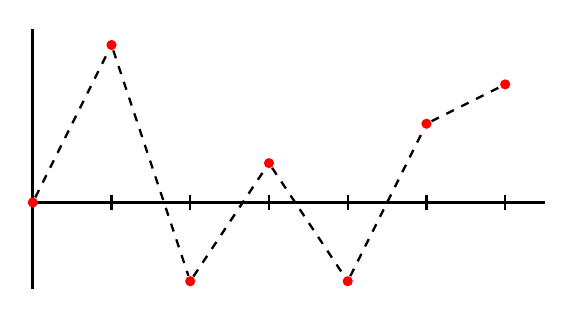
\begin{tikzpicture}
  \tikzset{
    pics/tick/.style args={#1}{code={
      \draw[line width=0.3mm] (0,-#1) -- (0,#1) ;
      },
    }
  }
  
    %AXIS Y
    \draw[line width=0.4mm] (0,-1.1) -- ++(90:3.3cm);
    %AXIS X 
    \draw[line width=0.4mm] (0,0) --++(0:6.5cm);
  
    \draw (0,0) pic {tick={1mm}} node[circle,inner sep=1.3pt,fill=red,yshift=0cm] (0) {};
    \draw (1,0) pic {tick={1mm}} node[circle,inner sep=1.3pt,fill=red,yshift=2cm] (1) {};
    \draw (2,0) pic {tick={1mm}} node[circle,inner sep=1.3pt,fill=red,yshift=-1cm] (2) {};
    \draw (3,0) pic {tick={1mm}} node[circle,inner sep=1.3pt,fill=red,yshift=0.5cm] (3) {};
    \draw (4,0) pic {tick={1mm}} node[circle,inner sep=1.3pt,fill=red,yshift=-1cm]  (4) {};
    \draw (5,0) pic {tick={1mm}} node[circle,inner sep=1.3pt,fill=red,yshift=1cm] (5) {};
    \draw (6,0) pic {tick={1mm}} node[circle,inner sep=1.3pt,fill=red,yshift=1.5cm] (6) {};
    \foreach \x/\y in {0/1,1/2,2/3,3/4,4/5,5/6} {
      \draw[dashed,line width=0.3mm] (\x) -- (\y) ;
    }
  \end{tikzpicture} 
  }
\end{center}
\end{figure}
Since there is no dependence between the values at different times the paths can look completely wild.  
		\item Here is a path of the so-called Brownian motion, indexed by $I=[0,\infty)$ that we will get to know later in this course.
			\begin{figure}[H]
				\input{./kapitel/Kapitel6/Bilder/ex_2_3_BM.tex}		
			\end{figure}
		\item A Poisson process is indexed by $I=[0,\infty)$ but mostly acts like a discrete-time process. The process jumps up by $1$ at independent exponentially distributed random variables of parameter $\lambda>0$. The parameter is called jump-intensity as a change in $\lambda$ result in more/less frequent jumps.
			
\begin{figure}[h]
		\begin{center}

  \tikzset{
    pics/tick/.style args={#1}{code={
      \draw[line width=0.3mm] (0,-#1) -- (0,#1) ;
      },
    }
  }
  % BLACK AXIS 
  \begin{tikzpicture}
    %AXIS Y
    \draw[black!90,line width=0.4mm] (0,-0.5) -- ++(90:2.5cm);
    %TICKS Y 
    \draw[black] (0,0.5) pic[rotate=90] {tick={1mm}} node[left,scale=0.8,xshift=-1mm] {1};
    \draw[black] (0,1) pic[rotate=90] {tick={1mm}} node[left,scale=0.8,xshift=-1mm] {2};
    \draw[black] (0,1.5) pic[rotate=90] {tick={1mm}} node[left,scale=0.8,xshift=-1mm] {3};
    %AXIS X 
    \draw[black!90,line width=0.4mm] (-0.5,0) --++(0:6.5cm);
    
    \draw[draw=darkgreen,line width=0.4mm] (0,0) -- (1,0) node[circle,inner sep=1pt,fill=darkgreen,pos=0] (S1) {};
    \draw[decorate,decoration={brace,mirror,raise=2mm},draw=darkgreen,line width=0.4mm,xshift=-0.1mm,scale=0.9] (0,0) -- (1,0) node[darkgreen,anchor=north,yshift=-5mm,pos=0.55,scale=0.8] {Exp($\lambda$)}; 

    \draw[draw=darkgreen,line width=0.4mm] (1,0.5) -- (3,0.5) node[circle,inner sep=1pt,fill=darkgreen,pos=0] (S2) {};
    \draw[decorate,decoration={brace,mirror,raise=2mm},draw=darkgreen,line width=0.4mm,xshift=-0.5mm,scale=0.98] (1,0) -- (3,0) node[darkgreen,anchor=north,yshift=-5mm,pos=0.55,scale=0.8] {Exp($\lambda$)}; 

    \draw[draw=darkgreen,line width=0.4mm] (3,1) -- (4,1) node[circle,inner sep=1pt,fill=darkgreen,pos=0] (S3) {};
    \draw[decorate,decoration={brace,mirror,raise=2mm},draw=darkgreen,line width=0.4mm,xshift=-0.5mm] (3,0) -- (4,0) node[darkgreen,anchor=north,yshift=-5mm,pos=0.55,scale=0.8] {Exp($\lambda$)}; 

    \draw[draw=darkgreen,line width=0.4mm] (4,1.5) -- (5.5,1.5) node[circle,inner sep=1pt,fill=darkgreen,pos=0] (S4) {};
    \draw[decorate,decoration={brace,mirror,raise=2mm},draw=darkgreen,line width=0.4mm] (4,0) -- (5.5,0) node[darkgreen,anchor=north,yshift=-5mm,pos=0.55,scale=0.8] {Exp($\lambda$)} ;
  \end{tikzpicture} 

\end{center}
\end{figure}		
						The Poisson process is called Poisson process as the so-called one-dimensional distributions $X_t$ are $\textrm{Poi}(\lambda t)$-distributed for all $t>0$.
		\item Markov chains are stochastic processes indexed by $\N$ or $\N_0$ (depending on taste).
			\end{enumerate}
\end{example}
We come now back to the discussion from Section \ref{sec:gentle} about $\sigma$-algebras and information in the context of stochastic processes.
\begin{ldef}
\begin{deff}
	Suppose $(\Omega, \mathcal F,\P)$ is a probability space and $I$ an index set.
	\begin{enumerate}[label=(\roman*)]
	\item An increasing family $\lbrace \cF_t \colon t \in I \rbrace $ of sub-$\sigma$-algebras of $\cF$, i.e $\cF_t \subseteq \cF_s$ for $t \leq s$, is called a \textbf{filtration}. 
%	\item A filtration is said to be \textbf{complete} if $\cF_t$ contains all $\mathbb{P}$-nullsets of $\cF$ for all $t\in I$.
%	\item A filtration is called \textbf{right-continuous} if $\cF_t = \cF_{t+} \coloneqq \bigcap_{s>t}\cF_s$. 
	\item A tuple $\big(\Omega,\cF,(\cF_t)_{t \in I},\mathbb{P}\big)$ is called a \textbf{filtered probability space}.
	\item We will frequently use the notation $\cF_{\infty}\coloneqq \sigma\big( \bigcup_{t\in I}\cF_t\big)\subseteq \mathcal F$.
	\end{enumerate}
\end{deff}
\end{ldef}
There are many filtrations for which we always use the interpretation that $\mathcal F_t$ contains the information someone gives us up to time $t$. The most important example in the study of stochastic processes is the natural filtration induced by a stochastic process:
\begin{ldef}
\begin{deff}\label{ex_ch2_2}
	Suppose $X$ is a stochastic process indexed by $I$, then 
	\begin{align*}
		\mathcal F_t:=\sigma(X_s:s\leq t), \quad t\in I,
	\end{align*}
	is called the \textbf{natural filtration of $X$} or the filtration generated by $X$.
\end{deff}
\end{ldef}
Recall the discussion from Section \ref{sec:gentle} if time and space $E$ are discrete. Since everything is countable we can write down $\mathcal F_n$ explicitly as
		\begin{align*}
		\mathcal F_n
		=\sigma\big(\{ \{X_1 \in A_1, ..., X_n \in A_n \} : A_i\subseteq E \}\big)
		=\sigma\big(\{\{X_1=i_1,..., X_n=i_n\}: i_k\in E \}\big).
	\end{align*}	
	We always interpret $\mathcal F_n$ as the information of $X$ up to time $n$ as precisely those events $A\in \mathcal F$ belong to $\mathcal F_n$ that can be written in terms of paths up to time $n$.
\begin{ldef}
\begin{deff}
	A stochastic process $(X_t)_{t\in I}$ is \textbf{adapted to a filtration} $(\cF_t)_{t\in I}$ if $X_t$ is $\cF_t$-measurable for all $t\in I$.
\end{deff}
\end{ldef}
If we recall from Section \ref{sec:gentle} the interplay of $\sigma$-algebras, measurability, and information the following interpretation should be kept in mind. If $X$ is adapted to a filtration, then the information of the filtration is enough to know $X$. A stochastic process is always adapted to it's natural filtration (it's own information) and to all bigger filtrations (even more information).\smallskip

\begin{lwarnhinweis}
From now on we will discuss discrete-time stochastic processes only equipped with the power set as $\sigma$-algebra. We will return to continuous-time processes when we introduce the Brownian motion. 
\end{lwarnhinweis}
While in discrete time the measure theory works analogously to finite time (finite product $\sigma$-algebras) the measure theory   becomes very involved in continuous time.

%\begin{deff}[Measurability concepts for processes]\label{deff_meas_concept_processes}
%	Let $X$ a stochastic process in continuous time, i.e. $I = \mathbb{R}_+$, on $\big(\Omega,\cF,(\cF_t)_{t \in I},\mathbb{P}\big)$.
%	\begin{enumerate}[label=(\roman*)]
%		\item
%			$X$ is called \textbf{measurable} if 
%			\begin{align*}
%				X^{-1}(A) = \lbrace (t,\omega)\colon X_t(\omega)\in A\rbrace \in \cB(\mathbb{R})\otimes\cF \:\:\:\: \forall A \in \varepsilon
%			\end{align*}
%		\item
%			$X$ is \textbf{progressively measurable} if, for every $t\geq 0$, the map 
%			\begin{align*}
%				[0,t]\times \Omega &\rightarrow E \\ 
%				(s,w) &\mapsto X_s(\omega)
%			\end{align*}
%			is $\cB\big( [0,t]\big) \otimes \cF_t$-$\varepsilon$-measurable.
%	\end{enumerate}
%\end{deff}
%(ii) $\Rightarrow$ (i), (i) $\not\Rightarrow$ (ii). But no worries: If $X$ is right-continuous the equality holds.
%\begin{lemma1}\label{lemma_prog_meas_if_right_cont}
%	Let $X$ be a continuous time process on $\big(\Omega,\cF,(\cF_t)_{t\in I},\mathbb{P}\big)$. If $X$ is right-continuous and $(\cF_t)$-adapted with values in $\big( \mathbb{R}^d,\cB(\mathbb{R}^d)\big)$, then $X$ is progressively measurable.
%\end{lemma1}
%\begin{proof}
%	Fix $t \geq 0$. For $n \in \mathbb{N}$,\,$s\leq t$ define 
%	\begin{align*}
%		X_s^{(n)}\coloneqq \begin{cases}
%			X_{\frac{k+1}{2^n}\cdot t} &, s\in \big[ \frac{k}{2^n}\cdot t ,  \frac{k+1}{2^n}\cdot t \big) \\
%			X_t &, s=t \end{cases}
%	\end{align*}
%	\begin{figure}[H]
%		\graphicspath{ {./kapitel/kapitel6//} }
%		\includegraphics[scale=0.5]{plot28}
%	\end{figure}
%	For any $B \in \varepsilon$ we have
%	\begin{align*}
%		&\{ ( s , \omega ) \in [0,t] \times \Omega | X_s^{(n)}( \omega )\in B \} \\
%		&= \bigcup\limits_{0 \leq k < 2^n}\Bigg(\underbrace{\bigg[\frac{k}{2^n}t,\frac{k+1}{2^n}t\bigg)}_{\in \cB([0,t])}\times \underbrace{\{\omega \colon  X_{\frac{k+1}{2^n}t}\in B \}}_{\in\cF_t} \Bigg)\cup \underbrace{\lbrace t \rbrace}_{\in\cB([0,t])} \times \underbrace{\lbrace \omega \, \colon \, X_t(\omega)\in B \rbrace}_{\in\cF_t}
%	\end{align*}	 
%	$\in \cB\big([0,t]\big) \otimes \cF_t$.
%	By right-continuity $X_s^{(n)}(\omega) \rightarrow X_s(\omega)$ for all $\omega \in \Omega$,\: $s\leq t$. Hence, \:$(s,\omega)\mapsto X_s^{(n)}$ is progressively measurable. Since measurability transfers to point-wise limits, also $(s,\omega) \mapsto X_s$ is progressively measurable.	
%\end{proof}

\begin{ldef}
\begin{deff}\label{def_stopping_time}
	Let $\big(\Omega,\cF,(\cF_n)_{n\in I},\mathbb{P}\big)$ be a filtered probability space.
	\begin{enumerate}[label=(\roman*)]
	\item	 A random variable $\tau\colon \Omega \rightarrow I \cup\lbrace +\infty \rbrace$ is called an \textbf{$(\cF_n)$-stopping time} if
	\[ \lbrace \tau \leq n \rbrace \in \cF_n \quad \forall n \in I \text{.}\]
	\item	$\tau$ is called a \textbf{finite stopping time} if $\tau < \infty $ a.s.
\end{enumerate}
\end{deff}
\end{ldef}
We usually think of a stopping time to model that something of interest happens at that time, for instance a given state is hit by the process. The idea of a stopping time is then easy to grasp: a random variable is called a stoping time if we only need information up to time $n$ to decided if $\tau$ happened before time $n$ or not.

\begin{remark}
	\begin{enumerate}[label=(\roman*)]
		\item It is important to allow $\tau=\infty$ with the interpretation  "{}the thing of interest did not happen"{}.
				\item	Since here we only work in discrete time we could also define a stopping time by asking $\{\tau=n\}\in \mathcal F_n$ for all $n\in I$. This follows easily from
%			\begin{align*}
%				\lbrace \tau < t \rbrace = \bigcup\limits_{n\in\mathbb{N}} \lbrace \tau \leq t-\frac{1}{n} \rbrace \in \cF_t \\
%				\lbrace \tau < t \rbrace = \lbrace \tau \leq t \rbrace \cap \lbrace \tau < t \rbrace^C \in \cF_t
%			\end{align*}
			\begin{align*}
				 \lbrace \tau \leq n \rbrace = \bigcup\limits_{k\leq n}\lbrace \tau = k \rbrace 
			\end{align*}
			because $\lbrace \tau = k \rbrace \in \cF_k \subseteq \cF_n$.
		\item
			A stopping time $\tau$ is not only $\mathcal F$-measurable but even $\cF_{\infty}$-measurable:
			\begin{align*}
				\lbrace \tau =n \rbrace=\lbrace \tau \leq n\}\cap \{\tau \leq n-1\}^C\in \cF_n\subseteq  \cF_{\infty}
			\end{align*}
			and
			\begin{align*}
				\lbrace \tau = \infty \rbrace = \lbrace \tau \neq \infty \rbrace^C = \big( \bigcup\limits_{n\in\mathbb{N}} \lbrace \tau = n \rbrace \big)^C \in \cF_{\infty}.
			\end{align*}	
	\end{enumerate}
\end{remark}
Even though we could formulate everything with $\{\tau =n\}$ we prefer to use $\{\tau \leq n\}$ in order to slowly get acquainted to a notion which cannot be avoided in continuous time.\smallskip


Here are the most important (and most simplistic) examples:
\begin{example}\label{ex_ch2_3}
%	Let $X$ be $(\cF_t)$-adapted.
\begin{lbeispiel}
	\begin{enumerate}[label=(\roman*)]
			\item 
			Every constant $\tau = N$ is a stopping time as $\{N \leq n\}\in \{\emptyset, \Omega\}\in \mathcal F_n$.

		\item
			Fix some $B\in \mathcal E$, then the \textbf{first hitting time} $\tau_B \coloneqq \inf\lbrace n \in I\,:|\, X_n \in B \rbrace$  is a stopping time as
			\begin{align*}
				\lbrace \tau_B \leq n \rbrace = \bigcup\limits_{k\leq n}\underbrace{\lbrace X_k \in B \rbrace}_{\in \mathcal F_k\subseteq \mathcal F_n} \in \cF_n.
			\end{align*}
%		\item 
%			$I = \mathbb{R}_+$,\:$E$ metric space, $\cO \subseteq E$ open,\:$F\subseteq E$ closed
%			\begin{itemize}
%				\item 
%					If $X$ is continuous, then $\tau_F = \inf\lbrace t\leq 0 \colon X_t \in \cO \rbrace$ is an $(\cF_t)$-stopping time
%				\item
%					If $X$ is right-continuous, then $\tau_{\cO} = \inf \lbrace t \geq 0 \colon X_t \in \cO \rbrace$ is an $(\cF_{t+})$-stopping time
%			\end{itemize}			
	\end{enumerate}
\end{lbeispiel}

\end{example}
Intuitively it is clear that the minimum of two stopping times ("{}one of the two events happened"{}) is a stopping time again. Please prove this as a short exercise:
\begin{luebung}
	If $T_1, T_2,...$ is a sequence of $(\cF_n)$-stopping times, then 
	\[ \inf_{k\in\N} T_k , \:\sup_{k\in\N} T_k , \:\liminf_{k\to\infty} T_k, \text{ and }\limsup_{k\to\infty} T_k \]
	are stopping times as well.
\end{luebung}
%\begin{proof}[Proof]
%	Using the definitions of the infimum and limit inferior we can directly check the definition. Fix $n\in I$, then
%	\begin{align*}
%		\{ \inf T_k \leq n \} = \bigcup\limits_{k=1}^{\infty}\underbrace{\{ T_k \leq n \}}_{\in \mathcal F_n}\in \cF_n
%	\end{align*}
%	and
%	\begin{align*}
%		\{ \liminf T_k \leq n \} = \bigcap\limits_{m=0}^{\infty}\bigcup\limits_{k=m}^{\infty}\underbrace{\{T_k \leq n \}}_{\in \cF_n} \in \cF_n.
%	\end{align*}
%	Hence, both are stopping times. For the limit inferior we used that the limit inferior is smaller than $n$ if and only if there are infinitely many $T_k$ which are smaller than $n$ which is equivalent to finding some $T_k$ which are smaller than $n$ after every fixed $m$. \smallskip
%Exercise	
%	The arguments for the supremum and limit superior are similar.
%\end{proof}





As mentioned above we interpret the natural filtration as information of the process, $\mathcal F_n$ as the information up to time $n$. We now generalise towards stopping times and give a mathematical definition of the information up to a stopping time.
\begin{ldef}
\begin{deff}
	Let $\tau$ be an $(\cF_n)$-stopping time. Then
	\begin{align*}
		\cF_{\tau}:= \lbrace A\in \cF_{\infty}\, :\, A \cap \lbrace \tau \leq n \rbrace \in \cF_n \:\: \forall n \in I \rbrace
	\end{align*}
	is called the $\mathbf{\sigma}$\textbf{-algebra generated by $\mathbf{\tau}$}
\end{deff}
\end{ldef}
It will need a bit of time to get used to $\mathcal F_\tau$. As always it is most instructive to have some examples in mind. Fix the first stopping time $\tau_B$ of a set $B$ and check by hands that for some other set $A$ the event "{}$A$ was hit before $B$"{} is in $\mathcal F_{\tau_{B}}$. This should intuitively be clear as only the process until first hitting $B$ is needed to decide if $A$ was already hit. 
\begin{llemma}
\begin{prop}\label{ii}
	Suppose $\tau$ is an $(\mathcal F_n)$-stopping time. 
	\begin{enumerate}[label=(\roman*)]
		\item 	$\cF_{\tau}$ is a $\sigma$-algebra on $\Omega$.
		\item	 	$\tau$ is $\cF_{\tau}$-measurable.
	\end{enumerate}
\end{prop}
\end{llemma}
\begin{proof}[Proof]
\begin{enumerate}[label=(\roman*)]
\item Let us check the defining properties of a $\sigma$-algebra:
	\begin{itemize}
		\item
			$\Omega \cap \lbrace \tau \leq n \rbrace \in \cF_n$, hence, $\Omega \in \mathcal F_\tau$.
		\item
			Let $A \in \cF_{\tau}$, then \[ A^C \cap \lbrace \tau \leq n \rbrace = \lbrace \tau \leq n \rbrace \cap \big( A \cap \lbrace \tau \leq n \rbrace \big)^C \in \cF_n \]
			so that $A^C\in \cF_\tau$.		
		\item
			Let $A_1,A_2,... \in \cF_{\tau}$, then
				\[ \bigcup\limits_{k=1}^{\infty}A_k \: \cap \lbrace \tau \leq n \rbrace = \bigcup\limits_{k=1}^{\infty} \underbrace{\left(A_k \cap \lbrace \tau \leq n \rbrace\right)}_{\in \cF_n}\in\cF_n \]
			so that $\cup_{k=1}^\infty A_k\in \mathcal F_\tau$.
	\end{itemize}
\item Exercise

\end{enumerate}
\end{proof}

Stopping times are useful as many properties of deterministic times also hold for stopping times.
\begin{llemma}
\begin{prop}\label{pS}
	Suppose $S, T$ are $(\cF_n)$-stopping times.
	\begin{enumerate}[label=(\roman*)]
		\item
			$S \leq T$\, a.s.\, $\Rightarrow\,$ $\cF_S \subseteq \cF_T$
		\item
			$\cF_{S\wedge T} = \cF_S \cap \cF_T$
		\item
			$\lbrace S \leq T \rbrace \in \cF_{S\wedge T}$ and $\lbrace S = T \rbrace \in \cF_{S\wedge T}$
%		\item
%			$S+T$ is an $(\cF_n)$-stopping time
	\end{enumerate}
\end{prop}
\end{llemma}
Before checking the proofs have a quick thought why those statements should intuitively be true with the interpretation of stopping times and the information given by a stopping time.
\begin{proof}[Proof]
	\begin{enumerate}[label=(\roman*)]
		\item
			\begin{align*}
				A \in \cF_S \quad &\Rightarrow \quad A \cap \lbrace S\leq n \rbrace \in \cF_n\,\, \forall n \in I \\
							&\Rightarrow \quad A \cap \lbrace T \leq n \rbrace = A \cap \lbrace S \leq n \rbrace \cap \lbrace T \leq n \rbrace \in \cF_n\,\,\forall n \in I\\
							&\Rightarrow  \quad A \in \cF_{T}
			\end{align*}
		\item We have seen above that $S\wedge T$ is an $(\mathcal F_n)$-stopping time again. Now towards the generalised $\sigma$-algebras:\smallskip
			
			"$\supseteq$": Let $A\in \cF_S\cap\cF_T$ and $n\in I$, then 
					\[ A \cap \{ S \wedge T \leq n \} = A \cap \big( \{ S \leq n \} \cup \{ T \leq n \} \big) =\big(A \cap  \{ S \leq n \} \big) \cup \big( A\cap \{ T \leq n \} \big) \in \cF_n \]
					Hence, $A \in \cF_{S\wedge T}$.\smallskip
				
			"$\subseteq$": This follows from the monotonicity proved in (i): $\cF_{S\wedge T} \subseteq \cF_s$, $\cF_{S\wedge T} \subseteq \cF_T$
		\item	Try yourself!		
	\end{enumerate}
\end{proof}
The definitions of stopping times and adapted processes work nicely together, here is an example:
\begin{llemma}
\begin{prop}\label{cha2_prop_X_tau_adapted}
	If $X$ is adapted to the filtration $(\cF_n)$ and $\tau$ is a finite $(\mathcal F_n)$-stopping time, then $X_{\tau}$ is $\cF_{\tau}$-measurable.
\end{prop}
\end{llemma}
\begin{proof}[Proof]
	The finiteness of $\tau$ was only assumed to make $X_\tau$ well-defined as we did not define $X_\infty$. Let $A \in \mathcal{E}$, we show $\lbrace X_{\tau} \in A \rbrace \in \cF_{\tau}$. Let $n\in I$, then
	\begin{align*}
		\lbrace X_{\tau} \in A \rbrace \cap \lbrace \tau \leq n \rbrace = \bigcup_{m\leq n}\underbrace{ \{ X_m \in A \} \cap \{ \tau = m \} }_{\in \mathcal F_m \subseteq \mathcal F_n}\in \cF_n
	\end{align*}
\end{proof}


	\marginpar{\textcolor{red}{Lecture 5}}
\section{Basics of martingales}

All processes in this chapter are indexed by discrete ordered sets such as $I = \mathbb{N}_0$, $I =\mathbb{N}$, $I=\Z$, $I=-\N$, or $I \subseteq \mathbb{N}$ and we write $n$ instead of $t$. We start the discussion of martingales with definitions and some first properties.

\begin{ldef}
\begin{deff}\label{def_martingale}
Let $I$ a discrete ordered index-set, $\big(\Omega , \cF , (\cF_n)_{n\in I}, \mathbb{P}\big)$ a filtered probability space, and $X=(X_n)_{n\in I}$ an $(\cF_n)_{n\in I}$-adapted process with $\E[\left| X_n \right| ] < \infty$ for all $ n \in I$. Then $X$ is called an
	\begin{enumerate}[label=(\roman*)]
		\item 
			$(\cF_n)_{n\in I}$\textbf{-martingale} if $\E[X_{n+1}\,|\,\cF_n]=X_n$ a.s. for all $n\in I$,
		\item
			$(\cF_n)_{n\in I}$\textbf{-supermartingale} if $\E[X_{n+1}\,|\,\cF_n] \leq X_n$ a.s. for all $ n\in I$,
		\item
			$(\cF_n)_{n\in I}$\textbf{-submartingale} if $\E[X_{n+1}\,|\,\cF_n] \geq X_n$ a.s. for all $ n\in I$.
	\end{enumerate}
	If $I=-\N$ or $I=-\N_0$ we will speak of a \textbf{backwards martingale}, for $I=\N$, $I=\N_0$, or $I=\{0,...,N\}$ of a \textbf{forwards martingale} but we will always skip the supplement forwards.
\end{deff}
\end{ldef}
The interpretation of a martingale is that of a fair game (this is where the name "{}martingale"{} comes from). Given the past value the expectation of profit in the next step is $0$. Analogously, a supermartingale is seen as an unfavourable game (we will loose in expectation) and submartingales are seen as favourable games. The power of martingales is astonishing. Most of the time they appear from nowhere in a context that does not look like a typical martingale setting and their powerful convergence theorems yield strong results. We will see as an example a proof of the law of large numbers without any additional assumption.\smallskip

Please check the following easy properties yourself!
\begin{luebung} 
	\begin{enumerate}[label=(\roman*)]
		\item The (sub)(super)martingale property also holds over several time steps:
		\begin{align*}
		 \E[X_m \, |\,\cF_n]\,\,
		\begin{cases}
			=X_n&: X\text{ martingale}\\
			\leq X_n&: X\text{ supermartingale}\\
			\geq X_n&: X\text{ supermartingale}
			\end{cases},
		\end{align*}
		for all $m\geq n$.
%			Why?
%			\begin{align*}
%				\E[X_m \,|\, \cF_n] &= \E \big[ \E [ X_m \, | \, \cF_{m-1}]\, | \, \cF_n \big] && \text{tower property}\\
%				&=\E[X_{m-1}\,|\,\cF_n] \\
%				&= ...&& \text{turn this into an induction!} \\
%				&= \E[X_{n+1}\,|\, \cF_n] = X_n
%			\end{align*}
		\item	Expectations (increase)(decrease)stay constant depending on $X$ being a (sub)(super)martingale:
		\begin{align*}
			\E[X_m] \,\,
			\begin{cases}
				=\E[X_n]&: X\text{ martingale}\\
				\leq \E[X_n]&:X\text{ supermartingale}\\
				\geq \E[X_n]&:X\text{ submartingale}\\				
			\end{cases},
		\end{align*}	
		for all $m\geq n$.
%			$\E[X_m] = \E[X_n], m \geq n$, if $(X_n)_{n\in\mathbb{N}}$ is a martingale, \\
%			$\E[X_m] \leq \E[X_n], m \geq n$, if $(X_n)_{n\in\mathbb{N}}$ is a supermartingale and \\
%			$\E[X_m] \geq \E[X_n], m \geq n$, if $(X_n)_{n\in\mathbb{N}}$ is a submartingale \\
%			Why? $\E[X_n] = \E \big[ \E[X_m\,|\,\cF_n] \big] = \E[X_m]$
		
		\item
			$X$ is a supermartingale $\Leftrightarrow$ $-X$ is a submartingale.
	\end{enumerate}
\end{luebung}
The final property allows us to prove theorems in most cases for either sub- or supermartingales and then transfer the theorems to the other.\smallskip

Even though the (super)(sub)martingale properties seems artificial many stochastic processes share this property:
\begin{example}
	The most prominent stochastic process in discrete time is the random walk which is a Markov chain and also a martingale.
	
\begin{figure}[h]
\begin{center}
\scalebox{0.8}{
  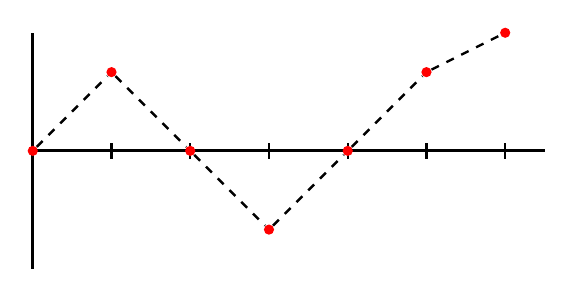
\begin{tikzpicture}
  \tikzset{
    pics/tick/.style args={#1}{code={
      \draw[line width=0.3mm] (0,-#1) -- (0,#1) ;
      },
    }
  }
    %AXIS Y
    \draw[line width=0.4mm] (0,-1.5) -- ++(90:3cm);
    %AXIS X 
    \draw[line width=0.4mm] (0,0) --++(0:6.5cm);

    \draw (0,0) pic {tick={1mm}} node[circle,inner sep=1.3pt,fill=red,yshift=0cm] (0) {};
    \draw (1,0) pic {tick={1mm}} node[circle,inner sep=1.3pt,fill=red,yshift=1cm] (1) {};
    \draw (2,0) pic {tick={1mm}} node[circle,inner sep=1.3pt,fill=red,yshift=0] (2) {};
    \draw (3,0) pic {tick={1mm}} node[circle,inner sep=1.3pt,fill=red,yshift=-1cm] (3) {};
    \draw (4,0) pic {tick={1mm}} node[circle,inner sep=1.3pt,fill=red,yshift=0cm]  (4) {};
    \draw (5,0) pic {tick={1mm}} node[circle,inner sep=1.3pt,fill=red,yshift=1cm] (5) {};
    \draw (6,0) pic {tick={1mm}} node[circle,inner sep=1.3pt,fill=red,yshift=1.5cm] (6) {};
    \foreach \x/\y in {0/1,1/2,2/3,3/4,4/5,5/6} {
      \draw[dashed,line width=0.3mm] (\x) -- (\y) ;
    }
  \end{tikzpicture} 
  }
  \end{center}
  \vspace{-4mm}
  \caption*{A trajectory of the simple random walk}
\end{figure}
	\begin{lbeispiel}		
	Let $Y_1,Y_2,Y_3,..$ be iid real-valued integrable random variable. The \textbf{random walk with jump sizes $Y_k$} is defined by $X_0:=x\in\R$ and 
			\begin{align*}
			 	X_n = x + \sum\limits_{k=1}^{n}Y_k, \quad n \in \mathbb{N}.
			\end{align*}
					If $\P(Y_1=1)=p$ and $\P(Y_1=-1)=1-p$ the random walk is called \textbf{simple random walk}, for $p=\frac 1 2$ symmetric simple random walk.
		\end{lbeispiel}
				\vspace{-2mm}

		
			If we define $\cF_0 = \lbrace \emptyset,\Omega \rbrace$ and $\cF_n = \sigma(Y_1,...,Y_n)$ then the random walk is an
			\begin{itemize}
				\item
					$(\mathcal F_n)$-martingale if $\E[Y_1]=0$,
				\item
					$(\mathcal F_n)$-supermartingale if $\E[Y_1] \leq 0$,
				\item
					$(\mathcal F_n)$-submartingale if $\E[Y_1] \geq 0$.
			\end{itemize}
			To see why, let us check the definition. Adaptivity and integrability ($\Delta$-inequality) is clear, the martingale property is deduced using properties of the conditional expectation:
			\begin{align*}
				\E[X_{n+1}\,|\,\cF_n] &= \E \big[ \sum\limits_{k=1}^{n+1}Y_k \,\big|\,\cF_n\big]\\
											&= \sum\limits_{k=1}^{n+1} \E[Y_k\,|\,\cF_n] \\
											&= \sum\limits_{k=1}^{n}Y_k \: + \: \E[Y_{n+1}\,|\,\cF_n]\\% && Y_k\:\text{is}\: \cF_n\text{-meas. for}\: k\leq n \\
											&= X_n + \E[Y_1],
			\end{align*}
			using in the third equality the measurability and independence assumption on the jump sizes.
\end{example}
\begin{example}\label{GW}		
 Another famous class of discrete time stochastic processes are so-called branching processes ("{}Verzweigungsprozesse"{}). 
\begin{lbeispiel}
	Let $\xi_i^n,\: i,n\in \mathbb{N}$, be integrable, non-negative discrete iid random variables with $\mathbb{P}(\xi_1^n=k) = p_k$, $k\in\mathbb{N}_0$. 
	The classical \textbf{branching process} (or \textbf{Galton-Watson process}) with offspring distribution $\xi$ is defined by
	\begin{align*}
		X_0 &\coloneqq m,\quad	X_{n+1} \coloneqq \sum_{k=1}^{X_n}\xi_k^n,\quad n\in\N.
	\end{align*}
	We will call $X_n$ the number of individuals of a population at time $n$.
\end{lbeispiel}
	\begin{figure}[h]
	\begin{center}
		\includegraphics[scale=0.12]{M2.jpeg}		
	\end{center}
		\vspace{-0.3cm}
	\caption*{Branching process with $m=3$ and extinction time $5$}
\end{figure}

	The interpretation goes as follows. At time zero there are $m$ individuals, plants for examples. At every time-unit, once a year for plants, every existing individual gets offspring. The number is independent from all offspring of other individuals in the same generation but also independent of the past. The genealogical picture is typically represented by a graph, $X_n$ counts the number of individuals at time $n$. We say the branching process gets extinct if $X_n=0$, after the first extinction time the process stays extinct forever. We always assume $p_0,p_1\neq 1$ as otherwise the branching process either dies out immediately ($p_0=1$ forces all initial individuals to have zero offspring) or stays constant ($p_1=1$ forces all individuals to have exactly one offspring so that $X_n=m$ for all $n\in\N$). Typical questions concern the probability of extinction or the rate of growth (exponential, subexponential). A critical feature is the mean number of offspring $\mu =\E[\xi_1^n] = \sum_{k=0}^{\infty}k\cdot p_k$ which is the main driver for the longtime behavior.\smallskip
	
	 If we define $\cF_0 = \lbrace \emptyset,\Omega \rbrace$ and $\cF_n = \sigma(\xi_i^k: i\in \N,k\leq n)$ then the branching process $X$ is an
			\begin{itemize}
				\item
					$(\mathcal F_n)$-martingale if $\mu=1$, called the \textbf{critical case},
				\item
					$(\mathcal F_n)$-supermartingale if $\mu<1$, called the \textbf{subcritical case},
				\item
					$(\mathcal F_n)$-submartingale if $\mu>1$, called the \textbf{supercritical case}.
			\end{itemize}
	Let us check the definition which is similar to the computation for the random walk except we need to deal with the random delimiter in the sums for which we need the Wald-identity:
	\begin{luebung}
		Suppose $N, Y_1,Y_2,...$ are independent, $\E[N]<\infty$, and $Y_1,Y_2,...$ are identically distributed, then
		\begin{align}\label{Wald}
			\E\Big[\sum_{k=1}^N Y_k\Big]=\E[N]\cdot \E[Y_1].
		\end{align}
	\end{luebung}
	Integrability is deduced immediately as the Wald-identity gives $\E[X_n]=\E[X_{n-1}]\cdot \E[\xi_1^1]$ so that $\E[X_n]=m\mu^{n}<\infty$ by a simple induction. Adaptivity follows direction from the definition of $\mathcal F_n$. The martingale property is deduced using properties of the conditional expectation:
			\begin{align*}
				\E[X_{n+1}\,|\,\cF_n] &= \E\big[ \sum_{k=1}^{\infty}\mathbf 1_{k \leq X_n}\cdot \xi_k^{n+1}\,\big|\,\cF_n\big] \\
										&=\sum_{i=1}^{\infty}\mathbf 1_{j \leq X_n} \E\big[\xi_j^{n+1}\,|\,\cF_n\big] \\
										&=\sum_{i=1}^{\infty}\mathbf 1_{j \leq X_n} \E\big[\xi_j^{n+1}\big] 
										=\mu \cdot X_n,
			\end{align*}
			using monotone convergence, measurability and the independence of conditional expectation. Interestingly, there is another martingale appearing in the branching process. If we define $M_n \coloneqq \frac{1}{\mu^n}\cdot X_n$, $n\in\N$, then $M$ is a martingale in all three regimes! Adaptivity and measurability is clear, the martingale property follows with the same calculation as above with an additional cancellation:			
			$$ \E[M_{n+1}\,|\,\cF_n] = \frac{1}{\mu^{n+1}}\cdot \E[X_{n+1}\,|\,\cF_n] = \frac{1}{\mu^{n+1}} \cdot \mu \cdot X_n = M_n.$$
			We already get a first impression of what is going by checking the expectations, which are constant for the martingale $M$. Then the expectations of $X_n$ remain constant for $\mu=1$ grow exponentially as $\mu^n=e^{\log(\mu)n}$ for $\mu>1$ and decay exponentially for $\mu<1$.
		\end{example}
\begin{example}\label{doobmartingale}
%\begin{enumerate}
%	\item
%			If $(X_n)_{n\in \mathbb{N}}$ is a generic integrable, $(\cF_n)$-adapted, decreasing (i.e. $X_n \geq X_{n+1}$ a.s.) process, then $(X_n)_{n\in\mathbb{N}}$ is an $(\cF_n)$-supermartingale as
%			\begin{align*}
%				 \E[X_{n+1}\,|\,\cF_n] \leq \E[X_n\,|\,\cF_n] = X_n \quad \text{a.s.}
%			\end{align*}
%			Similarly, an adapted increasing process is a submartingale.
%		\item
			If $Z$ is an integrable random variable on $(\Omega,\cF,\mathbb{P})$ and $(\cF_n)$ is a filtration, then $$X_n \coloneqq \E[Z\,|\,\cF_n],\quad n\in\N,$$ is a martingale. The argument is simple but very important:
			\begin{align*}
				\E[X_{n+1}\,|\,\cF_{n}] = \E \big[ \E[Z\,|\,\cF_{n+1}]\,\big|\,\cF_n \big] 
											\overset{\text{tower prop.}}{=} \E[Z\,|\,\cF_n] = X_n\quad \text{a.s.}
			\end{align*}
			Every martingale $(X_n)_{n\in\mathbb{N}}$ that can be written as $\E[Z\,|\,\cF_n]$ for some integrable random variable $Z$ is called a \textbf{closed martingale} or \textbf{Doob martingale}. It is best to think of a Doob martingale as a martingale on finite time horizon $\{0,...,N\}$ as in both cases one random variable ($Z$ for a Doob martinglae, $X_N$ for a finite-time martingale) determines the entire martingale. In the end of Section \ref{secL1} it will be shown that closed martingales (or, equivalently, uniformly integrable martingales) indeed share important properties of finite-time martingales.
%			
%			
%			We will think of $Z$ as the last element as we will later see the connection to the limit $X_\infty=\lim_{n\to\infty} X_n$. Doob martingales are useful as only one random variable $Z$ determines all random variables $X_n$, in a way, closed martingales are as simple as martingales on finite time-horizon $\{0,...,N\}$. It will be proved later that many martingales are Doob martingales!
%	\end{enumerate}

	\end{example}
\begin{llemma}
\begin{prop}\label{prop314}
	Let $\varphi \colon \mathbb{R} \rightarrow \mathbb{R}$ be a convex function, and $(X_n)_{n\in\mathbb{N}}$ a stochastic process with $\E[\left| \varphi(X_n)\right|] < \infty$.
	\begin{enumerate}[label=(\roman*)]
		\item
			If $(X_n)_{n\in\mathbb{N}}$ is an $(\cF_n)$-martingale, then $\big(\varphi(X_n)\big)_{n\in\mathbb{N}}$ is an $(\cF_n)$-submartingale.
			
		\item
			If $(X_n)_{n\in\mathbb{N}}$ is an $(\cF_n)$-submartingale and $\varphi$ is increasing, then $\big(\varphi(X_n)\big)_{n\in\mathbb{N}}$ is an $(\cF_n)$-submartingale.
	\end{enumerate}
\end{prop}
\end{llemma}
\begin{proof}
	We use Jensen's inequality for conditional expectation:
	\begin{enumerate}[label=(\roman*)]
		\item
			$\E \big[\varphi(X_{n+1})\,|\,\cF_n\big] \geq \varphi \big( \E[X_{n+1}\,|\,\cF_n]\big) = \varphi(X_n)$ a.s. The equality uses the martingale property.
		\item
			$\E \big[\varphi(X_{n+1})\,|\,\cF_n\big] \geq \varphi \big( \E[X_{n+1}\,|\,\cF_n]\big) \geq \varphi (X_n)$ a.s. The second inequality uses that $\varphi$ is increasing and the submartingale property.
	\end{enumerate}
\end{proof}
As usual, the simplest examples are the most useful ones. One can regularly see the use of $\varphi (x) = \left| x \right|$, $\varphi (x) = (x-a)^+ $, and powers $\varphi (x) = \left| x \right|^p$ for $p \geq 1$.
\begin{lwarnhinweis}
	Most importantly, $(X_n^2)_{n\in\N}$ is a submartingale if $(X_n)_{n\in\mathbb{N}}$ is a martingale with $\E[X_n^2]<\infty$ for all $n\in\N$.
\end{lwarnhinweis}
Here is something simple to check yourself. 
\begin{luebung}
	Suppose $(X_n)_{n\in\mathbb{N}}$ and $(Y_n)_{n\in\mathbb{N}}$ are $(\cF_n)$-martingales.
	Then the sum $(X_n+Y_n)_{n\in\mathbb{N}}$ is an $(\cF_n)$-martingale and the maximum $(X_n \vee Y_n)_{n\in\mathbb{N}}$ is an $(\cF_n)$-submartgingale.
\end{luebung}
%\begin{proof}
%$\E[X_{n+1}+Y_{n+1} \, | \, \cF_n ] = \E[X_{n+1}\,|\,\cF_n]+\E[Y_{n+1}\,|\,\cF_n] \geq X_n + Y_n$ a.s.\\
%$\E[X_{n+1}\vee Y_{n+1}\,|\,\cF_n] \geq \E[X_{n+1}\,|\,\cF_n] \geq X_n$ a.s. and \\
 %$\E[X_{n+1}\vee Y_{n+1}\,|\,\cF_n] \geq \E[Y_{n+1}\,|\,\cF_n] \geq Y_n$.\\ Hence, $\E[X_{n+1}\vee Y_{n+1}\,|\,\cF_n] \geq X_{n+1}\vee Y_{n+1}$ a.s.
%\end{proof}
We come to the first theorem on martingales where we relate martingales and stopping times. If $T$ is a stopping time then we define the \textbf{stopped process} $X^T$ as $$X_n^T(\omega)\coloneqq X_{n \wedge T(\omega)}(\omega),\quad n \in \mathbb{N}.$$ The path of the stopped process is the same as the original process up to time $T$ and stays constant at the value $X_T$ after time $T$. 
\begin{figure}[h]
  \begin{center}
  \scalebox{0.7}{
  \begin{tikzpicture}
  \tikzset{
    cross/.pic ={
      \draw[pic actions,rotate=#1,line width=0.3mm] 
        (-3pt,0) -- (3pt,0)
        (0,-3pt) -- (0,3pt);
    },
  }
  \tikzset{
    pics/tick/.style args={#1}{code={
      \draw[line width=0.3mm] (0,-#1) -- (0,#1) ;
      },
    }
  }
  %AXIS Y
  \draw[black,line width=0.4mm] (0,-0.5) -- ++(90:4.5cm);
  %AXIS X 
  \draw[black,line width=0.4mm] (-0.5,0) --++(0:9cm); 
  \foreach \x in {1,2,...,8}{
    \draw (\x,0) pic {tick={1mm}} ;
  }
  \foreach \x/\y in {1/1,2/2,3/1.5,4/2.5,5/2}{
    \draw (\x,\y) pic {cross={0}} node[inner sep=0mm] (\x) {};
    \draw[violet] (\x,\y) pic {cross={45}};
  }
  \draw[violet] (5,0) pic {tick={1mm}};

  
  \definecolor{darkViolet}{RGB}{74,2,104}
  \draw[violet] (6,2) pic {cross={45}} node[] (6) {} ;
  \draw[violet] (7,2) pic {cross={45}} node[] (7) {};
  \draw[violet] (8,2) pic {cross={45}} node[] (8) {};

  \foreach \x/\y in {0/1,1/2,2/3,3/4,4/5,5/6,6/7,7/8} {
      \draw[dashed,line width=0.2mm,draw=darkViolet] (\x) -- (\y) ;
    }

  \draw (6,3)   pic {cross={0}}node[inner sep=0.5mm] (6) {};
  \draw (7,2.5) pic {cross={0}}node[inner sep=0.5mm] (7) {};
  \draw (8,3.5) pic {cross={0}}node[inner sep=0.5mm] (8) {};

  \draw[dashed,line width=0.2mm,draw=black] (5) -- (6) ;
  \draw[dashed,line width=0.2mm,draw=black] (6) -- (7) ;
  \draw[dashed,line width=0.2mm,draw=black] (7) -- (8) ;


  %TEXT 
  \node[violet,yshift=-4mm] (stopT) at (5,0) {$T$};

  \node[black] (blackPath) at  (9,3.5) {$X$} ;
  \node[violet,yshift=-4mm,xshift=1mm] (violetPath) at (blackPath.south)  {$X^T$};
  \end{tikzpicture}
  }
\vspace{-2mm}
\caption*{Path of a stopped process $X^T$}
\end{center}
\end{figure}
It might be instructive to realise that stopping at deterministic times $T=N$ shows how to relate infinite time-horizon martingales to finite time-horizon martingales on $\{0,...,N\}$.\smallskip

The optional stopping theorem states that a martingale stopped at a stopping time (i.e. without future information) remains a martingale. We can derive as an application the so-called optional sampling theorem. The theorem formalises the idea of a fair game that without future information it is impossible to reach a gain in expectation by stopping. While we will see after the theorem an example that this statement is a bit too optimistic it does hold for bounded stopping times:
\begin{lsatzwichtig}
\begin{theorem}[Optional Stopping/Optional Sampling Theorem]\label{optional_stopping}
	Suppose $(X_n)_{n\in\mathbb{N}}$ is an $(\cF_n)$-martingale and $T$ is an $(\cF_n)$-stopping time.
	\begin{enumerate}[label=(\roman*)]
		\item The \textbf{stopped process} $(X_n^T)_{n\in\N}$ is an $(\cF_n)$-martingale.
		\item
			If $T$ is a \textbf{bounded} $(\cF_n)$-stopping time, i.e. $\mathbb{P}(T \leq K ) = 1$ for some $K\in \mathbb{N}$, then $X_T$ is an integrable random variable with $\E[X_T] = \E[X_1]$.
	\end{enumerate}
\end{theorem}
\end{lsatzwichtig}
The optional sampling theorem in particular applies to martingales on finite time-horizon $\{0,...,N\}$ when the optional sampling theorem is applied to the stopped martingale $X^N$.



\begin{proof}[Proof]
	We mainly prove the optional stopping theorem, optional sampling is a direct consequence.\smallskip
	
	\textbf{Optional Stopping Theorem:} 
			We check the three defining properties (adapted, integrable, martingale property):
			\begin{itemize}\label{(i)}
				\item 
					First note that $n\wedge T$ is a stopping time (minimum of two stopping times), hence, $X_{n\wedge T}$ is $\cF_{n \wedge T}$-measurable by Proposition \ref{cha2_prop_X_tau_adapted}. Since $\cF_{n\wedge T} \subseteq \cF_n$ by Proposition \ref{pS}, $X^T$ is $(\cF_n)$-adapted.
				\item The integrability of $X^T$ follows by splitting on the possible values of $T$:
				\begin{align*}
						\E\big[| X_n^T |\big] &= \E \Big[ \left| X_{n \wedge T} \right|  \sum\limits_{k=1}^{\infty}\mathbf 1_{T=k} \Big]\\
						&\leq \E \Big[\sum\limits_{k=1}^{n} \left| X_{k} \right|  \mathbf 1_{T=k} \Big]+\E \Big[\sum\limits_{k={n+1}}^{\infty } \left| X_{n} \right|  \mathbf 1_{T=k} \Big]\\				
						&\leq \E \Big[\sum\limits_{k=1}^{n} \left| X_{k} \right| \Big]+\E \big[\left| X_{n} \right| \mathbf 1_{T\geq n+1}\big]\\				
						&\leq \sum\limits_{k=1}^{n} \E [| X_{k} | ]+\E [\left| X_{n} \right| ]<\infty.
				\end{align*}					
				\item To show the martingale property we use a trick that will return frequently. To show the martingale property it is enough to show that the differences are so-called martingale differences:
				\begin{ltippwichtig}
					Trick: $(X_n)_{n\in\mathbb{N}}$ is an $(\cF_n)$-martingale iff $\E[X_{n+1}-X_n\,|\,\cF_n]=0$ a.s. for all $n\in\N$. 
				\end{ltippwichtig}
				To justify the martingale difference trick one only needs to use the linearity of conditional expectation and that $X$ is adapted.\smallskip
				
				Let's check that the differences of $X^T$ are martingale differences:
					\begin{align*}
						\E\big[X_{n+1}^T-X_n^T\,\big|\,\cF_n\big] &= \E \big[ (X^T_{n+1}-X^T_n)(\mathbf 1_{T\leq n}+\mathbf 1_{T > n})\,\big|\,\cF_n\big] \\
						&= \E\big[(X_{n+1}-X_n) \mathbf 1_{T > n}\,\big|\,\cF_n\big] \\
						&= \mathbf 1_{T>n} \E[X_{n+1}-X_n\,|\,\cF_n] 
						= 0
					\end{align*}
					where we used that
					\begin{itemize}
						\item
							$X_{n+1}^T=X_n^T$ on the event $\lbrace T \leq n \rbrace$,
						\item
							$X_{n+1}^T = X_{n+1}, X_n^T = X_n$ on $\lbrace T > n \rbrace$,
						\item
							$\mathbf 1_{T>n}$ is measurable as $\lbrace T>n \rbrace = \lbrace T\leq n\rbrace^C \in \cF_n$ by the stopping time property.
					\end{itemize}
			\end{itemize}
			
			\textbf{Optional Sampling Theorem:} 
			Using that the stopped martingale is again a martingale and that martingales have constant expectations we obtain the theorem:
			\begin{align*}
				\E[X_T] \overset{T\leq K}{=} \E[X_{K\wedge T}] =\E[X_{K}^T]=\E[X_1^T] = \E[X_{T \wedge 1}] = \E[X_1].
			\end{align*}				
\end{proof}
\begin{lwarnhinweis}
	The boundedness of $T$ can be weakend but not generally be removed! Always keep in mind the random walk example below as a counter example!
\end{lwarnhinweis}

\begin{remark}
	\begin{enumerate}[label=(\roman*)]
		\item
		The boundedness assumption on $T$ can be removed if $X$ is bounded! If $T$ is a finite stopping time, then $$\E[X_T] = \E\big[ \lim\limits_{n \to \infty} X_{T\wedge n}\big] \overset{\text{DCT}}{=} \lim\limits_{n \to \infty}\E[X_{T\wedge n}] \overset{\text{mart.}}{=} \lim\limits_{n \to \infty} \E[X_1] = \E[X_1].$$
		\item
		The boundedness assumption on $T$ can be weakend to $\E[T] < \infty$ if the martingale differences are almost surely bounded, i.e. $\lvert X_n - X_{n+1}\rvert \leq K$ almost surely for all $n\in\N$. In that case it holds that 
		\begin{align*}
			\lvert X_T- X_{T \wedge n}  \rvert \overset{\text{telescope}}= \Big| \sum\limits_{k=T\wedge n }^{T-1} (X_{k+1}-X_k)\Big| \leq K\cdot T
		\end{align*}
		so that, again by dominated convergence, we obtain
		$$\lim\limits_{n \to \infty}\big(\E[X_{T}]-\E[X_{\wedge n}]\big) =  \E\big[\lim\limits_{n \to \infty}(X_{T}-X_{T\wedge n})\big] = \E[0] = 0.$$ 
		Since $\E[X_{T\wedge n}]=\E[X_1] $ by optional stopping, optional sampling follows.
				\item As a counter example to the optional sampling theorem when the boundedness of $T$ is violated let us consider the symmetric simple random walk. Let $T = \inf\{n\in\mathbb{N}\colon X_n=1\}$ and $X_0=0$. Then $T<\infty$ almost surely but $$\E[X_T] = 1 \neq 0 = \E[X_0] = \E[X_n]$$ for $n\in \mathbb{N}$. Since the martingale differences are bounded (they are $+1$ or $-1$), (ii) shows that $\E[T]=\infty$.

	\end{enumerate}
\end{remark}
The random walk example is the first time we can feel the power of martingales. It was quite easy to prove $\E[T]=\infty$ via the option sampling theorem. But how can you prove this by hands? Just try to compute $\P(T=k)$ for some $k$ and you will see that you run quickly into combinatorics.


 Of course you could try to do this by hands by 

\begin{ldef}
\begin{deff}
	A stochastic process $(H_n)$ is called \textbf{previsible} (or \textbf{predictable}) if $H_n$ is $\cF_{n-1}$-measurable. (\enquote{$H_n$ only depends on information up to $n-1$}). 
	\end{deff}
\end{ldef}
\footnote{Leif: Indexmengen aufraeumen}
Previsibility is actually quite a natural concept. If for instance $H_n$ could be the amount you want to invest at day $n$ based upon the price of the day $n-1$ before. Such concepts are clearly important in mathematical finance but also in probability theory.
\begin{ldef}
\begin{deff}
 Suppose $(X_n)_{n\in\mathbb{N}_0}$ is an $(\cF_n)$-adapted stochastic process and $(H_n)$ is $(\cF_n)$-predictable, then we define 
	\begin{align*}
		(H\cdot X)_0 &\coloneqq 0,\\
		(H\cdot X )_n &\coloneqq \sum\limits_{k=1}^{n}H_k \cdot (X_k - X_{k-1}).
	\end{align*}
	Since $H \cdot X$ is the discrete analog of stochastic integral $\int_{0}^{t}H_s \dint X_s$ we call $H\cdot X$ the \textbf{discrete stochastic integral of $H$ agains $X$}.
\end{deff}
\end{ldef}
The interpretation of $H\cdot X$ in mathematical finance is the wealth obtained by trading the asset $X$ using the trading strategy $H$. Here is bad news: If your favorit asset is a martingale and you only have a bounded amount of money to invest, there is no way of making money by clever stopping (in your life time) your investment. Unfortunately, $H\cdot X$ will always be a martingale so that the expectation will be constant at all bounded stopping times by the optional sampling theorem.
	\marginpar{\textcolor{red}{Lecture 6}}

\begin{lsatz}
\begin{theorem}[Sorry, but you really cannot beat the system.]\label{you_cannot_beat_the_system}
	Suppose $(H_n)$ is predictable and bounded (i.e. $\lvert H_n\rvert \leq K$ a.s. for all $n\in \N$).
	\begin{enumerate}[label=(\roman*)]	
		\item
			If $X$ is a martingale, then $H\cdot X$ is  a martingale.
		\item
			If $X$ is a supermartingale and $H \geq 0$, then $H\cdot X$ is a supermartingale.
		\item
			If $X$ is a submartingale and $H \geq 0$, then $H\cdot X$ is a submartingale.	
	\end{enumerate}
\end{theorem}
\end{lsatz}
\begin{proof}
	\begin{enumerate}[label=(\roman*)]	
		\item We need to check the three defining properties of a martingale.
			\begin{itemize}
				\item
					$(H\cdot X)_n$ is $\mathcal F_n$-adapted by definition
				\item Since $H$ is bounded by assumption and $X$ is integrable as a martingale we obtain
				\begin{align*}
					\E\big[|(H\cdot X )_n|\big] \overset{\Delta}{\leq}  \sum\limits_{k=1}^{n}\E\big[|H_k \cdot (X_k - X_{k-1})|\big] \leq K \sum_{k=1}^n (\E[|X_k|]+\E[|X_{k-1}|])<\infty.
				\end{align*}
							\item
				The martingale property follows from a direct computation using the assumed measurability properties to simplify the conditional expectations:
					\begin{align*}
						\E\big[ (H\cdot X)_{n+1}\,\big|\,\cF_n\big] &= \E \Big[ \sum\limits_{k=1}^{n+1} H_k (X_k-X_{k-1})\,\Big|\, \cF_n \Big] \\
						&=\sum\limits_{k=1}^{n} H_k(X_k-X_{k-1}) + \E\big[ H_{n+1}(X_{n+1}-X_n)\,\big|\,\cF_n\big] \\
						&= (H\cdot X)_n+0,\quad \text{a.s.}
					\end{align*}
					The last equation holds, because $H$ is predictable and $\E[X_{n+1}-X_n\,|\,\cF_n]=0$ almost surely by the martingale property.
			\end{itemize}
		\item
			Since $\E[X_{n+1}-X_n\,|\,\cF_n]\leq 0$ a.s. for a supermartingale and $H \geq 0$ we can replace the last equation from our calculation above with $\leq$.
		\item
			Just like (ii).
	\end{enumerate}
\end{proof}
In this probability theory lecture we will not care about mathematical finance, but nonetheless, the discrete stochastic integral will be a massively useful tool for us! We can for instance give an alterntive proof for optional stopping by using the previous theorem with $H_n \coloneqq \mathbf 1_{T\geq n} = 1 - \mathbf 1_{T<n}$. $H$ is previsible and $X_{n\wedge T}$ can be rewritten as
$$ X_{n\wedge T} = (H\cdot X)_n + X_0$$ because $$ (H\cdot X)_n = \sum\limits_{k=1}^{n}\mathbf 1_{T\geq k}(X_k - X_{k-1}) = X_{n\wedge T} - X_0 $$
Hence, $(X_{n\wedge T})_{n\in\N}$ is a martingale. Similar tricks of playing with the discrete stochastic integrals will appear later. To prove the almost sure martingale convergence theorem and the optional sampling theorem for uniformly integrable martingales.

\section{Martingale convergence theorems}
The most striking feature of martingales is the rich convergence theory. Under very mild assumptions we will prove convergence
\begin{align*}
	X_n\to X_\infty,\quad n\to\infty,
\end{align*}
to some limiting random variable $X_\infty$, where the mode of convergence depends on the assumptions on $X$. As an example, without any further knowledge a non-negative martingale converges almost surely to a limit $X_\infty$. In the following sections we will discuss almost sure, $L^p$, and $L^1$ limit theorems.\smallskip

For the convergence theorems we will need a first element and an open end in the forwards direction for the limit to be interesting. The theorems work equally with $\N$ or $\N_0$, to have a consistent notation we will work with $\N_0$.



\subsection{Almost sure martingale convergence theorem}
We start with the most prominent martingale convergence theorem, the almost sure convergence theorem:
\begin{lsuperwichtigersatz}
\begin{theorem}[Almost sure martingale convergence theorem]\label{as}
	If $(X_n)_{n\in\mathbb{N}_0}$ is a (sub)martingale with $\sup_{n\in\mathbb{N}_0}\E[X_n^+]<\infty$, then almost surely $$X_{\infty} \coloneqq \lim_{n\to \infty}X_n $$ exists, is $\mathcal F_\infty$ measurable and almost surely finite with $\E[\lvert X_{\infty}\rvert]<\infty$.
\end{theorem}
\end{lsuperwichtigersatz}
The most useful application is towards non-negative martingales as they always satisfy the assumption of the almost sure martingale convergence theorem:
\begin{lsatz}
\begin{corollary}\label{MMM}
	If $(X_n)_{n\in\mathbb{N}_0}$ is a \underline{non-ne\smash{g}ative} martingale, i.e. $X_n\geq 0$ a.s. for all $n\in\N_0$, then almost surely $X_n$ converges to a limit $X_{\infty}$ with $0\leq \E[X_{\infty}] \leq \E[X_0]$.
\end{corollary}
\end{lsatz}
\begin{proof}
 The martingale property yields $ 0\leq \E[X_n^+] = \E[X_n] = \E[X_0] < \infty$ for all $n\in\N_0$ so that the almost sure martingale convergence theorem applies. Using Fatou's lemma then gives $$\E[X_{\infty}] = \E\big[ \lim_{n\to\infty}X_n \big] \leq  \liminf_{n\to \infty} \E[X_n] = \E[X_0].$$
\end{proof}
Here is the idea of the proof. 
\begin{lstep}
In order to have convergence of a real-valued sequence $(a_n)$ to a real number or infinity it is enough to prove that all intervals $[a,b]$ with rational endpoints are crossed only finitely many times.
\end{lstep}
The case of convergence towards infinity is clear, for a finite limit the claim is best seen by its contraposition. If a sequence does not converge, there are $a,b\in\mathbb Q$ such that $\liminf_n a_n< a<b<\limsup_n a_n$. Hence, the sequence $(a_n)$ takes infinitely many values larger than $b$ and smaller than $a$. But then the interval is crossed infinitely often. The martingale convergence theorem is proved by showing that the expected number of crosses through arbitrary intervals is finite, hence, the crossing number is almost surely finite. In fact, to prove that there are finitely many crossings it is enough to show that there are only finitely many upcrossings from below $a$ to above $b$.
%\begin{figure}[H]
%	\graphicspath{ {./kapitel/Kapitel6//} }
%	\includegraphics[scale=0.5]{plot321}
%\end{figure}
More formally, we define the crossing times by
\begin{align*}
	S_1 &\coloneqq 0 \\
		T_1 &\coloneqq \min\lbrace n\in \mathbb{N}_0: X_n \geq b \rbrace \\
	S_{k+1} &\coloneqq \min\lbrace n > T_k: X_n \leq a \rbrace \\
	T_{k+1} &\coloneqq \min\lbrace n > S_k: X_n \geq b \rbrace
\end{align*}
and set $$U_n[a,b]\coloneqq \sum\limits_{k=1}^{\infty}\mathbf 1_{T_k \leq n},$$ which is the number of finished upcrosings up to time $n$. The main ingredient towards the convergence theorem is the following estimate for the number of upcrossings:
\begin{llemma}
\begin{lemma}[Doob's upcrossing inequality]\label{upcrossing_inequality}
	If $(X_n)_{n\in\mathbb{N}_0}$ is a (sub)martingale and $a<b$, then $$ \E\big[ U_n[a,b]\big] \leq \frac{\E\big[ (X_n-a)^+ - (X_0-a)^+ \big]}{b-a}.$$
\end{lemma}
\end{llemma}
\begin{proof}[Proof]



			\begin{figure}[H]
				\includegraphics[scale=0.4]{mart2.jpeg}
				\vspace{-5mm}
				\caption*{Realisation of $X$ with four upcrossings and the counting using $H$, $Y$, and $H\cdot Y$}
			\end{figure}	


	In order to count the number of upcrossings we introduce 	 
	\begin{align*}
		Y_n&:= \max\{X_n,a\}=(X_n-a)^++a,\\
		H_n &\coloneqq \sum\limits_{k=1}^{\infty}\mathbf 1_{\{S_k<n\leq T_k\}}=\begin{cases}1&: n\in \{S_k+1,...,T_k\}\text{ for some }k\\0&:n\in \{T_k+1,...,S_k\}\text{ for some }k \end{cases}.
	\end{align*}	
	Additionally, we are interested in the discrete stochastic integral $H\cdot Y$. The idea of the proof is best understood through the illustration of the processes. We have chosen $H$ such that $H$ only takes the values $1$ and $0$ so that $H\cdot Y$ either stays constant (in intervals with $H=0$) or sums up the increments of $Y$. Every upcrossing of $X$ yields an increase of $H\cdot Y$ of at least $b-a$ so that $H\cdot Y$ counts (up to a factor $b-a$) the number of upcrossings.\smallskip
	
	Let's have a more formal look a the definitions. The telescopic sum property is best seen at the endpoints of upcrossings by removing all $0$ summmands:
			\begin{align*}
				(H\cdot Y)_{T_n} &=  \sum_{k=1}^{T_n}H_k(Y_k-Y_{k-1}) \\
							&= \sum_{k=1}^{n}\sum_{j=S_k+1}^{T_k}1\cdot (Y_j-Y_{j-1}) \\
							\overset{\text{telescope}}&{=} \sum_{k=1}^{n}(Y_{T_k}-Y_{S_k})	\\
							&\geq n\cdot (b-a)
			\end{align*}
			because $Y_{T_k}\geq b$ and $Y_{S_k} \leq a$. Now let us have a look at the values of $H\cdot Y$ in the two different ranges of the definition of $H$:			
		\begin{align*}
			(H\cdot Y)_j \overset{\text{adding }0s}{=} (H\cdot Y)_{T_n}\geq n(b-a),\quad \forall  j\in\lbrace T_n, \cdots,S_{n+1}\rbrace
		\end{align*}
		and, using this equality again,
		\begin{align*}
			(H\cdot Y)_j \overset{\text{telescope}}{\geq} (H\cdot Y)_{S_{n+1}} \overset{\text{adding }0s}{=} (H \cdot Y)_{T_n}\geq n(b-a),\quad\forall j\in \lbrace S_{n+1},\cdots,T_{n+1}-1 \rbrace.
		\end{align*}
	Noting that $j\geq T_n$ is the same as $n\geq U_j[a,b]$ (recall the definitions of $T_n$ and $U_j[a,b]$) we obtain
	\begin{align*}
		(H\cdot Y)_n \geq (b-a)U_n[a,b],\quad n\in\N_0.
	\end{align*}
	We are now close to finishing the proof using a submartingale argument. First note that $Y$ is a submartingale by Proposition \ref{prop314} as $x\mapsto (x-a)^++a$ is a convex function. Next, $H_n$ is previsible as $\mathbf 1_{\{S_k<n\leq T_k\}} = \mathbf 1_{\{S_k<n\}}\cdot \mathbf 1_{\{T_k<n\}^C}$ and sums and limits of measurable functions are measurable (compare \ref{hilf} and \ref{mlimits}). Hence, also $1-H_n$ is previsible so that  the discrete integral $(1-H)\cdot X$ is a submartingale by Theorem \ref{you_cannot_beat_the_system} because $1-H_n$ is bounded by $1$ and non-negative. But then, using that submartingales have increasing expectation, we obtain the desired bound:
	\begin{align*}
		\E[Y_n - Y_0] \overset{\text{telescope}}&{=} \E[(1\cdot Y)_n]\\
		 &= \E[(H\cdot Y)_n] + \E[((1-H)\cdot Y)_n]\\ 
		 \overset{\text{see above}}&{\geq} (b-a) \E\big[ U_n[a,b]\big] +  \E[((1-H)\cdot Y)_n] \\
		 \overset{(1-H)\cdot Y \text{ submart.}}&{\geq} (b-a) \E\big[ U_n[a,b]\big] + \E\big[ ( (1-H)\cdot Y )_0\big] \\
		&= (b-a) \E\big[ U_n[a,b]\big] + 0.
	\end{align*}
	Dividing by $b-a$ and plugging-in the definition of $Y$ yields the upcrossing inequality.
\end{proof}
With the upcrossing lemma we can quickly finish the proof of the martingale convergence theorem. The proof looks much worse than it is!
\begin{proof}[Proof of the almost sure martingale convergence theorem]
	Let $a<b$. Since $(X_n-a)^+ \leq \lvert a \rvert + X_n^+$ the upcrossing inequality gives $$ \E\big[ U_n[a,b]\big] \leq \frac{a+\E[X_n^+]}{b-a}$$
	and the right hand side is bounded by some $C<\infty$ due to the assumption on the submartingale. Now define
	\begin{align*}
		U[a,b]:=\lim_{n\to\infty} U_n[a,b]\in [0,\infty],
	\end{align*}	
	which is the total number of upcrossings through $[a,b]$. The limit exists as monotone sequences converge (with possible limit $+\infty$). Since the limit is monotone in $n$ we can use the monotone convergence theorem to obtain
	\begin{align*}
		\E\big[ U_n[a,b]\big] = \lim_{n\to \infty}\E\big[U_n[a,b]\big] \leq C.
	\end{align*}
	Since non-negative random variables with finite expectation are finite almost surely, we proved that $$\mathbb{P}(U[a,b]< \infty )=1,\quad \text{ for all }a<b.$$ Hence, we proved that almost surely the submartingale only crosses $[a,b]$ finitely often. If we define
	\begin{align*}
		C^{a,b} := \lbrace \omega: U[a,b](\omega) = \infty \rbrace \quad \text{and}\quad
		C := \bigcup_{a,b\in\mathbb{Q},\: a<b}C^{a,b},
	\end{align*}
	then the above shows that $\mathbb{P}(C^{a,b}) = 0$ and, hence, $\mathbb{P}(C)=0$. Since $C^C$ is the event that $X$ does not cross any interval infinitely often (equivalently, $X_n$ converges) and $\P(C^C)=1$ we proved that $\lim_{n\to\infty} X_n$ exists almost surely (with a possibly infinite limit).\smallskip
	
	Now define $X_\infty:=\lim_{n\to\infty} X_n$. Since all $X_n$ are $\cF_{\infty}$-measurable, $X_{\infty}$ is $\cF_{\infty}$-measurable as a limit. If we can show that $\E[|X_\infty|]<\infty$, then $X_\infty$ is finite almost surely. To show this we use Fatou's lemma twice. First, 
	\begin{align*}
		\E[X_{\infty}^-] \leq \liminf_{n\to\infty} \E[X_n^-] 
								= \liminf_{n\to\infty} \big( \E[X_n^+]-\E[X_n]\big) 
								\leq \sup_{n\in\N_0} \E[X_n^+] - \E[X_0] < \infty
	\end{align*}
	and, secondly,
	\begin{align*}
		\E[X_{\infty}^+] \leq \liminf_{n\to\infty} \E[X_n^+] <\infty.
	\end{align*}
	Hence, $\E[\lvert X_{\infty}\rvert ] < \infty$ and in particular $\lvert X_{\infty} \rvert < \infty$ a.s.
\end{proof}
A typical example for the martingale convergence theorem is a better understanding of the regimes in the branching process from Example \ref{GW}.
\begin{example}\label{branching1}
Recall the martingale $M$ obtained from the branching process which is actually a non-negative martingale. Hence, by Corollary \ref{MMM} there is a finite almost sure limit $M_{\infty}$ of $M_n$ which directly translates into knowledge on $X$. Here is an important fact that we use: If a sequence with values on $\N_0$ converges, then the sequence must ultimately be constant.
			\begin{enumerate}[label=(\roman*)]	
				\item 
				$\mu < 1$ (subcritical case): \\
					$\frac{1}{\mu^n} \to \infty$, so that $X_n = \mu^n M_n \to 0$, $n \to \infty$. But then the population modelled by $X$ suffers extinction in finite time almost surely, that is, almost surely gets absorbed at $0$ after some (unknown) random time $N(\omega)$.
				\item
					$\mu = 1$ (critical case): \\
					$(X_n)_{n\in\mathbb{N}}$ itself is a non-negative martingale so that $X_n \to X_{\infty}$ a.s. But how could the branching process stop moving ultimately? Right, only by almost sure extinct of the population in finite time (check the definition).
				\item
					$\mu > 1$ (supercritical case): \\
					Again the martingale convergence theorem implies
					$$\frac{1}{\mu^n}\cdot X_n \to M_{\infty}\in [0,\infty).$$
					Unfortunately, so far do not know anything about $M_\infty$ except being finite. On the event $E:=\lbrace\omega: M_{\infty}(\omega)> 0 \rbrace$ we observe exponential growth of the population, namely, $$X_n(\omega) \sim M_\infty(\omega) \mu^n = M_\infty (\omega) e^{\log(\mu)\cdot n}.$$ So far we cannot say if $E$ has positive probability. Under a square-integrability condition we will solve this question using the $L^2$-martingale convergence theorem below.
			\end{enumerate}
			What we see is an effect everyone learnt during the Covid pandemic. Sick people infecting on average more than $1$ person can lead to exponential growth, infecting on average less than $1$ person leads to extinction of the disease. Of course, this model is very simplistic due to the iid assumption on the offspring.
			
\end{example}
	\marginpar{\textcolor{red}{Lecture 7}}

\subsection{$L^p$-martingale convergence theorem for $p>1$}
After the almost sure convergence we now look for stronger conditions on martingales that additionally ensure convergence of $X_n$ towards $X_\infty$ in $L^p$, i.e. $\lim_{n\to\infty}\E[|X_n-X_\infty|^p]=0$. If you forgot about the $L^p$-spaces of random variables (modulo zero sets) with the norms $||X||_p=\E[|X|^p]^{1/p}$ please check Theorem \ref{Lp} and the discussion around. In this and the following section bounded sets in $L^p$ and $L^1$ will play a crucial role. Recall from analysis that bounded subsets of a normed space are subsets that lie in a ball with respect to the norm. In a sketchy picture (ignoring the linear structure) the situation looks as follows. 
\begin{figure}[h]
\begin{center}
  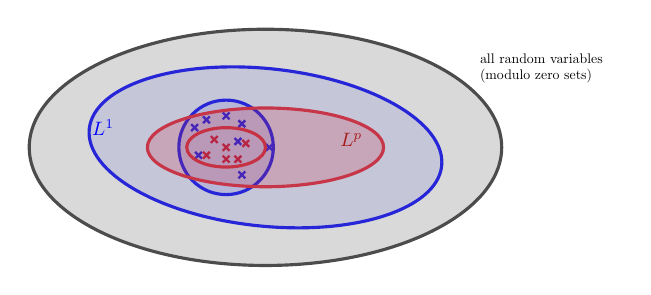
\begin{tikzpicture}[scale=0.5,transform shape]
  \tikzset{
    cross/.pic ={
      \draw[pic actions,rotate=#1,line width=0.3mm]
        (-3.5pt,0) -- (3.5pt,0)
        (0,-3.5pt) -- (0,3.5pt);
    },
  }
  \definecolor{darkred}{RGB}{168,27,27};
  \foreach \x/\y in {-1/0.8, -1.5/0.7, -1.8/0.5 , -0.6/0.6 , 0.1/0, -0.6/-0.7 , -1.7/-0.2,-0.7/0.15} {
    \draw (\x,\y) pic[blue] {cross={45}};
  } 
  \foreach \x/\y in {-1/0, -1.3/0.2,-1.5/-0.2,-1/-0.3,-0.7/-0.3,-0.5/0.1}{
    \draw (\x,\y) pic[red] {cross={45}};
  } 
  \draw[draw=blue!100,line width=0.4mm,fill=blue,fill opacity=0.1,rotate=0] (-1,0) ellipse (1.2 and 1.2);
  \draw[draw=red!90,line width=0.4mm,fill=red,fill opacity=0,rotate=0] (-1,0) ellipse (1 and 0.5);
  \draw[draw=red!90,line width=0.4mm,fill=red,fill opacity=0.2,rotate=0] (0,0) ellipse (3 and 1);
  \draw[draw=blue!100,line width=0.4mm,fill=blue,fill opacity=0.1,rotate=-6] (0,0) ellipse (4.5 and 2);
  \draw[draw=black!70,line width=0.4mm,fill=gray,fill opacity=0.3] (0,0) ellipse (6 and 3) ;
  \node[black,text width=3.5cm] at (7.2,2) {all random variables (modulo zero sets)};
  \node[blue,text width=2cm,scale=1.4] at (-3,0.5) {$L^1$};
  \node[darkred,text width=2cm,scale=1.4] at (3.3,0.2) {$L^p$};
  \end{tikzpicture} 
  \caption*{A schematic drawing of bounded sets of random variables in $L^p$ and $L^1$}
  \end{center}
\end{figure}
In this section we will show that martingales that are bounded in $L^p$ automatically converge in $L^p$ to a limit $X_\infty$. This feature of martingales is very special as typically one should not hope for convergence of a sequence only from knowing it is bounded. Martingales are just amazing!\smallskip




%Recall that convergence in $L^p$ means $\lim_{n\to\infty}\E[|X_n-X_\infty|^p]=0$. But since convergence in normed spaces implies convergence of the norms (norms are continuous) we would obtain $\lim_{n\to\infty}\E[|X_n|^p]=\E[|X_\infty|^p]$. So the very least one should assume to hold is boundedness of the $p$th moments as otherwise convergence is impossible. One of the magic features of martingales is that this condition is also enough. \smallskip

The estimates we develop are almost more important than the theorem itself, most importantly, Doob's inequalities for the so-called running supremum $X^*:=\max_{k\leq n} X_k$ appears in many places of probability theory. We start with a continuation of the optional sampling theorem:
\begin{llemma}
\begin{lemma}\label{lemma331}
	Let $(X_n)_{n\in\mathbb{N}_0}$ be an $(\cF_n)$-(sup)martingale and $S$, $T$ bounded $(\cF_n)$-stopping times with $S \leq T$ almost surely. Then
	\begin{enumerate}[label=(\roman*)]	
		\item
			$\E[X_S] \leq \E[X_T]$
		\item
			$\E[X_T\,|\,\cF_s] \geq X_s$, i.e. the (sup)martingale property also holds at bounded stopping times.
	\end{enumerate}
\end{lemma}
\end{llemma}
\begin{proof}
	\begin{enumerate}[label=(\roman*)]	
		\item The first claim is left as an exercise:
		\begin{luebung}
		Do you remember the proof of the optional sampling theorem sketched below Theorem \ref{you_cannot_beat_the_system}? The same trick can be used here using $H_n = \mathbf 1_{S < n \leq T}$. Do it!
		\end{luebung}
		\item First recall a general fact: If $X$ is a random variable on $(\Omega,\cA,\mathbb{P})$ with $\int_A X \dint \mathbb{P} \geq 0$ for all $A \in \cA$, then $X \geq 0 $ a.s. This follows directly by using the sets $A=\{X\leq 0\}$ and Theorem \ref{S7} (iii).\smallskip
		
		To use this fact we show $*$ in		
			\begin{align*}
				\E\big[ \E[ X_T\,|\,\cF_S]\mathbf 1_A \big] \overset{\text{cond. exp.}}{=} \E[X_T \mathbf 1_A] \overset{*}{\geq} \E[X_S \mathbf 1_A],\quad \forall A \in \cF_S
			\end{align*}
			because this implies $ \E[( \E[X_T\,|\,\cF_S]-X_S )\mathbf 1_ A ] \geq 0$ for all $A \in \cF_S$ and thus, using the fact above, $\E [X_T\,|\, \cF_S]\geq X_S$ a.s.  \smallskip
			
			To show $*$ fix $A\in \mathcal F_S$ and define $\tau_A= S\cdot \mathbf 1_A+T\cdot  \mathbf 1_{A^C}$. Then, $\tau_A$ is an $(\cF_n)$-stopping time (check the definition for yourself!). Finally, checking cases $\omega \in A$ and $\omega \in A^C$ for the first equality yields
			\begin{align*}
				\E[X_T] \overset{\text{(i)}}{\geq} \E[X_{\tau_A}] &= \E[X_T - X_T \mathbf 1_A + X_S  \mathbf 1_A] 
				= \E[X_T] - \E[X_T \mathbf 1_A] + \E[X_S \mathbf 1_A]
			\end{align*}
			which yields * by rearranging the inequality.
	\end{enumerate}
\end{proof}
We can use the lemma to prove an important theorem on martingales (or submartingales). Tail probabilities of the running maximum $X^*=\max_{k\leq n}X_n$ can be estimated with last element $X_n$ of the maximum. The inequality is not only important to prove limit theorems but appears at many places in probability theory or mathematical finance. 
\begin{lsatz}
\begin{theorem}[Doobs's maximal inequality]\label{Doobs_inequality}
	Let $(X_n)_{n\in\mathbb{N}_0}$ be an $(\cF_n)$-(sub)martingale and $\lambda > 0$. If $X_n^* \coloneqq \max_{k \leq n} X_k$ denotes the running maximum process, then the following inequalities hold:
	\begin{align*}
		\lambda \cdot \mathbb{P}(X_n^* \geq \lambda ) \leq \E[ X_n \mathbf 1_{\{X_n^* \geq \lambda\}}] \leq \E[X_n^+]
	\end{align*}
\end{theorem}
\end{lsatz}
To understand better the formula it might be useful to compare with the Markov inequality. Using the Markov inequality with $h(x)=x^+$ would yield $\E[(X^*_n)^+]$ on the right hand side which is potentially much bigger than the expectation of only the last random variable.

\begin{proof}[Proof]
	Let $T \coloneqq \min\{ n\in\mathbb{N}_0 \colon X_n \geq \lambda \}$ which is an $(\cF_n)$-stopping time so that $$A \coloneqq \{ X_n^*\geq \lambda \} = \{T \leq n \} \in \cF_n$$ and  $ \E[X_{T\wedge n}] \leq \E[X_n]$ by  Lemma \ref{lemma331}.
	  Now we write $$ X_{T \wedge n} = X_T \mathbf 1_{T \leq n}+ X_n \mathbf 1_{T>n}\geq \lambda \mathbf 1_{T \leq n} + X_n \mathbf 1_{T > n}$$ to get
	\begin{align*}
		\E[X_n] \geq \E[X_{T\wedge n}] &\geq \lambda \cdot \mathbb{P}(T\leq n) + \E[X_n \mathbf 1_{T>n}] 
		=\lambda \,\mathbb{P}(T\leq n) + \E[X_n] - \E[X_n \mathbf 1_{T\leq n}]
	\end{align*}
	which implies the first inequality: $$\lambda\, \mathbb{P}(X_n^* \geq \lambda) = \lambda \,\mathbb{P}(T \leq n ) \leq \E[X_n \cdot \mathbf 1_{X_n^*\geq \lambda}]$$
	The second inequality follows immediately from the first: $$ \E[X_n \mathbf 1_{X_n^*\geq \lambda}] \leq \E[X_n^+\mathbf 1_{X_n^*\geq \lambda}] \leq \E[X_n^+]$$
\end{proof}
We now turn the tail estimates into moment estimates by writing the moments as integrals over the tail probabilities.
\begin{lsatz}
\begin{theorem}[Doob's $L^p$-maximum inequality]\label{max_inequality}
	Suppose $p$ is a constant that is \underline{strictly} larger than $1$.
	\begin{enumerate}[label=(\roman*)]
		\item
			If $(X_n)_{n\in\mathbb{N}_0}$ is a non-negative $(\cF_n)$-(sub)martingale, then $$ \E\big[ \max\limits_{k \leq n} X_n^p\big] \leq \bigg(\frac{p}{p-1}\bigg)^p \E[X_n^p], \quad n\in \mathbb{N}_0.$$
		\item
			If $(Y_n)_{n\in{\mathbb N}_0}$ is an $(\cF_n)$-martingale, then $$ \E\big[ \max\limits_{k \leq n} \lvert Y_n\rvert^p \big] \leq \bigg(\frac{p}{p-1}\bigg)^p \E[\lvert Y_n\rvert^p],\quad n\in \mathbb{N}_0.$$
	\end{enumerate}
\end{theorem}
\end{lsatz}
Keep your eyes open to see why the proof cannot be modified in any way for $p=1$. The corresponding theorem for $p=1$ will be proved in the next section and is much harder.
\begin{proof}
	\begin{enumerate}[label=(\roman*)]
		\item The proof is just a clever computation keeping in mind that expectations can always be written as integrals over tail probabilities (Fubini, compare also proof of Theorem \ref{zusatz} or the exercises of Stochastik 1):
			\begin{align*}
				\frac{1}{p}\E\big[(X_n^*)^p\big] &= \E \Big[ \int_0^{X_n^*} \lambda^{p-1}\dint\lambda \Big] \\
												\overset{\text{Fubini}}&{=} \int_0^{\infty} \lambda^{p-2}\cdot \lambda \cdot\mathbb{P}(X_n^* \geq \lambda)\dint \lambda \\
												\overset{\text{\ref{Doobs_inequality}}}&{\leq}\int_0^{\infty} \lambda^{p-2} \E[X_n\mathbf 1_{X_n^*\geq \lambda}]\dint \lambda \\
												\overset{\text{Fubini}}&{=} \E \Big[ X_n \int_0^{\infty}\lambda^{p-2}\mathbf 1_{X_n^*\geq \lambda}\dint\lambda \Big] \\
												&= \E \Big[ X_n \int_0^{X_n^*}\lambda^{p-2}\dint \lambda \Big] \\
												&= \frac{1}{p-1}\E \big[ X_n \cdot (X_n^*)^{p-1}\big] \\
												\overset{\text{H\"older}\: q = \frac{p}{p-1}}&{\leq} \frac{1}{p-1} \E\big[(X_n)^p\big]^{\frac{1}{p}} \E\big[(X_n^*)^p\big]^{\frac{p-1}{p}}
			\end{align*}
			Dividing both sides gives the result.
		\item
			follows from (i) as $X_n \coloneqq \lvert Y_n \rvert$ is a submartingale
	\end{enumerate}
\end{proof}
As announced at the beginning of this section we will need to impose a stronger assumption on martingales in order to strengthen the almost sure convergence to $L^p$-convergence. A good condition is uniform $L^p$-boundedness:
\begin{ldef}
\begin{deff}
	A martingale is called $L^p$-martingale if $\sup_{n\in\mathbb{N}_0}\E[\lvert X_n \rvert^p] < \infty$. Most importantly, for $p=2$ we speak of square-integrable martingales.
\end{deff}
\end{ldef}
It is very important to keep in mind that the definition does not require finiteness of all $p$th moments but uniform boundedness of $p$th moments. Modulo zero sets this means the random variables of the martingale form a bounded set in the normed space $(L^p,||\cdot||_p)$. Since $(|X_n|^p)_{n\in\N_0}$ is a submartingale we know that $n\mapsto \E[X_n^p]$ is increasing, possibly towards $+\infty$. For $L^p$-martingales the sequence of $p$th moments does not grow to $+\infty$ but has a finite limit.\smallskip

We can now prove that $L^p$-boundedness is not only a necessary but also a sufficient condition for the $L^p$-convergence of martingales. The equivalence is not true for other sequences of random variables, we heavily use the martingale property.
\begin{lsuperwichtigersatz}
\begin{theorem}[$L^p$-martingale convergence theorem]
Suppose $p$ is a constant that is \underline{strictly} larger than $1$ and $(X_n)_{n\in\mathbb{N}_0}$ is an $L^p$-martingale. 
	\begin{enumerate}[label=(\roman*)]
		\item There is a (finite) limiting random variable $X_{\infty}\in \cL^p$ such that
		\begin{itemize}
			\item $X_n \overset{\text{a.s.}}{\to} X_{\infty}$ for $n \to \infty$,
			\item $X_n \overset{L^p}{\to}X_{\infty}$ for $n \to \infty$.
		\end{itemize}
			\item $\E\big[\lvert X_{\infty}\rvert^p\big] = \lim\limits_{n\to \infty}\E\big[\lvert X_n \rvert^p\big] = \sup\limits_{n\in\mathbb{N}_0} \E\big[\lvert X_n \rvert^p\big] < \infty$
			\item $\E\big[\sup\limits_{n\in\mathbb{N}_0}\lvert X_n \rvert^p\big] \leq \big(\frac{p}{p-1}\big)^p \cdot \E\big[\lvert X_{\infty}\rvert^p\big] < \infty$
	\end{enumerate}	
\end{theorem}
\end{lsuperwichtigersatz}
\begin{proof}[Proof]
\begin{enumerate}[label=(\roman*)]
	\item The first step is simple, using the simple estimate
	\begin{align*}
		x^+ \leq \lvert x \rvert^p + 1,\quad x\in\R.
	\end{align*}		
	Hence, every $L^p$-martingale satisfies the condition $\sup_{n\in\mathbb{N}_0} \E[X_n^+]<\infty$ of the martingale convergence theorem. Then there is a (finite) almost sure limit $X_{\infty}$. It remains to show that $X_\infty \in \mathcal L^p$ and the $L^p$-convergence. There is a simple thought to keep in mind, which also helps to appreciate Doob's inequalities:
	\begin{lstep}
		If $\sup_{k\in\N_0}|X_k|^p$ is integrable, than this is the perfect upper bound for dominated convergence. 
	\end{lstep}
	To check the integrability of the upper bound we use Theorem \ref{max_inequality}
	\begin{align*}
		\E\big[\lvert X_k^* \rvert^p\big] &\leq \left(\frac{p}{p-1}\right)^p \E\big[\lvert X_k\rvert^p\big] 
										\leq \left(\frac{p}{p-1}\right)^p \sup\limits_{n\in\mathbb{N}_0} \E\big[\lvert X_n\rvert^p\big],\quad \forall k\in \N_0,
	\end{align*}
	and monotone convergence:
	\begin{align*}
		\E\big[\big| \sup_{k\in \N_0} X_k\big|^p\big] = \E\big[\lim\limits_{k\to\infty}\lvert X_k^*\rvert^p\big]
										\leq \lim_{k\to\infty} \bigg(\frac{p}{p-1}\bigg)^p \E\big[\lvert X_k\rvert^p\big] < \infty.
	\end{align*}
	Hence, $\sup_{k\in \N_0} X_k\in \cL^p$ from which we immediately deduce $X_\infty \in \cL^p$ because $|X_\infty|\leq \sup_{k\in\N_0}|X_k|$. For the $L^p$-convergence first note that
	\begin{align*}
		\lvert X_n - X_{\infty} \rvert^p \leq (|X_n| +\lim_{n\to\infty} |X_n|)^p\leq  2^p \sup_{k\in \N_0} |X_k|^p\quad \text{for all } n\in \mathbb N_0,
	\end{align*}	
	and the right hand side is integrable. Then we can apply dominated convergence to the sequence of the left hand side:
	\begin{align*}
		\lim_{n\to \infty} \E\big[\lvert X_n - X_{\infty}\rvert^p\big] = \E\big[\lim_{n\to\infty}\lvert X_n - X_{\infty}\rvert^p\big] = \E[0] = 0.
	\end{align*}
	\item The first equality follows from basic functional analysis as convergence in a normed space implies convergence of norms: $\lim_{n\to\infty} ||X_n-X||= 0$ $\Rightarrow$ $\lim_{n\to\infty} ||X_n||=||X||$ because norms are continuous functions. Keeping in mind that $L^p$ is a normed space (modulo zero sets) we immediately find 
	\begin{align*}
		\E\big[\lvert X_{\infty}\rvert^p\big] = \lim_{n\to\infty} \E\big[\lvert X_n \rvert^p\big].
	\end{align*}
	The second equality follows from the monotonicity of $n\mapsto \E[|X_n|^p]$ as $(|X_n|^p)_{n\in \N_0}$ is a submartingale.
	\item
	The inequality follows from monotone convergence and Doob's $L^p$-maximal inequality:
	\begin{align*}
		\E\Big[ \sup\limits_{n\in\mathbb{N}_0} \lvert X_n \rvert^p \Big]
		&= \lim_{n\to\infty} \E \Big[ \sup\limits_{k\leq n} \lvert X_k \rvert^p \Big] 
		\leq \lim_{n\to\infty} \left( \frac{p}{p-1} \right)^p \E\big[\lvert X_n \rvert^p\big]
		\overset{(ii)}{=} \left( \frac{p}{p-1} \right)^p \E\big[\lvert X_{\infty} \rvert^p\big]
	\end{align*}
	\end{enumerate}
\end{proof}

	We come back to the branching processes as prime example for the convergence of martingales. The almost sure convergence of $M$ towards a finite limit $M_\infty$ was already checked. In the supercritical case we left open if $M_\infty$ is trivial, i.e. almost surely equal to $0$, or not. We can solve this question under the additional assumption that the offspring number has finite second moment.
\begin{example}\label{br2}
Let us additionally assume $\sigma^2:=\V[\xi_1^1]<\infty$, i.e. the offspring numbers have finite second moments. To keep things easy we assume $m=1$, there is one individual at time $0$. Wald's identity was used to compute first moments, to compute second moments of random sums one can first prove the Blackwell-Girshick identity:
	\begin{luebung}
		Suppose $N, Y_1,Y_2,...$ are independent, $\E[N]<\infty$, and $Y_1,Y_2,...$ are identically distributed, then
		\begin{align}\label{Wald2}
			\E\Big[\Big(\sum_{k=1}^N Y_k\Big)^2\Big]=\E[N]\V[Y_1]+\E[N^2]\E[Y_1]^2.
		\end{align}
	\end{luebung}
	Hence, we can compute the second moments of the martingale $M_n=\mu^{-n} X_n$:
	\begin{align*}
		\E\big[M_n^2\big]= \frac{1}{\mu^{2n}}\big(\mu^{n-1} \sigma^2+\E\big[X_{n-1}^2\big]\mu^2\big)=\frac{\sigma^2}{\mu^{n+1}} +\E\big[M_{n-1}^2\big]
	\end{align*}
	By induction this iteration gives
	\begin{align*}
		\E\big[ M_n^2\big]= \frac{\sigma^2}{\mu} \sum_{k=1}^{n} \mu^{-k} +1
	\end{align*}
	which increases for $\mu>1$ (geometric series) to a finite positive number. Hence, for $\mu>1$ we deduce $L^2$-convergence and, most importantly, $\E[M_\infty^2]=\lim_{n\to\infty} \E[M_n^2]>0$. But this implies $M_\infty>0$ with positive probability. If now we compare with Example \ref{branching1} we proved that the supercritical branching processes can increase exponentially fast with positive probability.

\end{example}



\subsection{$L^1$-martingale convergence theorem}\label{secL1}
	\marginpar{\textcolor{red}{Lecture 8}}
	We proved that $L^p$-bounded martingales converge automatically almost surely and in $L^p$ to a limit $X_\infty$. How about the same theorem for $p=1$? Unfortunately, the story is more complicated. The right condition for convergence in $L^1$ is not $L^1$-boundedness but a slightly stronger condition, so-called uniform integrability. To be honest, the world would be too simple if $L^1$-boundedness would be enough as otherwise every non-negative martingale would not only converge almost surely but also in $L^1$ as expectations of martingales are constant. But this cannot be as $\E[X_\infty]=\E[0]=0\neq \E[X_0]$ for the critical branching processes.
\begin{ldef}
\begin{deff}
	A familiy $(X_{\alpha})_{\alpha \in I}$ of random variables on $(\Omega,\cF,\mathbb{P})$ indexed by a set $I\neq \emptyset$ is called \textbf{uniformly integrable} if
	\begin{itemize}
		\item
			$\E[\lvert X_\alpha \rvert]< \infty$  for all $\alpha \in I$,
		\item
			$\lim\limits_{M \to \infty}\Big( \sup\limits_{\alpha \in I} \E\left[ \lvert X_{\alpha}\rvert \cdot \mathbf 1_{\lvert X_{\alpha}\rvert \geq M }\right]\Big) = 0$.
	\end{itemize}
\end{deff}
\end{ldef}
All the trouble about understanding this section is that we do not have simple examples to keep in mind. Everything is about abstract integration theory.
\begin{example}\label{exui}
	At least we have some classes of random variables that we are used to work with:
	\begin{enumerate}[label=(\roman*)]
		\item Families consisting of only one integrable random variable $\{X\}$ are uniformly integrable. This is easy:
			\begin{align*}
				 \lim_{M \to \infty} \E[\lvert X \rvert \mathbf 1_{\lvert X \rvert \geq M}] \overset{\text{DCT}}{=} 0
			 \end{align*}
			 The same holds for finite families:
			 \begin{luebung}
				Check that every finite number of integrable random variables forms a uniformly integrable family.
			\end{luebung}
		\item Every family of random variables that is dominated by an integrable random variable is uniformly integrable. We know this situation very well from the dominated convergence theorem! Suppose $\lvert X_{\alpha} \rvert \leq Z$ a.s. for all $\alpha\in I$ and $\E[\lvert Z \rvert] < \infty$, then
			\begin{align*}
				\lim_{M\to\infty}\sup\limits_{\alpha \in I}\E\big[\lvert X_{\alpha}\rvert \cdot \mathbf 1_{\lvert X_{\alpha}\rvert \geq M}\big] \leq \lim_{M\to\infty}\E[Z \cdot \mathbf 1_{Z\geq M}] \overset{\text{DCT}}{=} 0,\:\: M \to \infty
			\end{align*}
		\item
			If $(X_{\alpha})_{\alpha\in I}$ is bounded in $L^p$ for some $p>1$, i.e. $\sup_{\alpha\in I} \E[\lvert X_{\alpha}\rvert^p] < C$, then $(X_{\alpha})_{\alpha \in I}$ is also uniformly integrable. We will later use this situation to compare the $L^1$-convergence theorem to the $L^p$-convergence theorem of the previous section. To proof the claim let us first use the H\"older inequality with $p$ and $M$ fixed:
			\begin{align}\label{furchtbar}
				\E[\lvert X_{\alpha}\rvert \mathbf 1_{\lvert X_{\alpha}\rvert \geq M}] \leq \big( \E[\lvert X_{\alpha}\rvert^p]\big)^{\frac{1}{p}} \big(\E[\mathbf 1_{\lvert X_{\alpha}\rvert \geq M}]\big)^{\frac{1}{q}}\leq C^{1/p}\, \big(\P({\lvert X_{\alpha}\rvert \geq M})\big)^{\frac{1}{q}}.
			\end{align}
			We use the inequality to argue indirectly and assume the right hand side does not converge to zero uniformly in $\alpha$. If there is $\varepsilon > 0$ with $\liminf_{M\to \infty}\sup_{\alpha\in I}\E[\lvert X_{\alpha}\rvert \mathbf 1_{\lvert X_{\alpha}\rvert \geq M}] > \varepsilon$, then there is a sequence $\alpha_M$ with $\mathbb{P}(\lvert X_{\alpha_M}\rvert \geq M) > (\frac{\varepsilon}{2 C^{1/p}})^q$. But then
			\begin{align*}
				\E\big[\lvert X_{\alpha_M}\rvert^p \big] \geq  \E \big[ \lvert X_{\alpha_M}\rvert^p \mathbf 1_{\lvert X_{\alpha_M}\rvert \geq M}\big] \geq \Big(\frac{\varepsilon}{2 C^{1/p}}\Big)^q \cdot M^p \to \infty, \quad M \to \infty,
			\end{align*}
			which is a contradiction to $L^p$-boundedness. Hence, the right hand side of \eqref{furchtbar} goes to zero for all $M$. But then also the left hand side goes to zero for all $M$, which is exactly the uniform integrability.
	\end{enumerate}
\end{example}
\begin{ldef}
\begin{deff}
	A martingale is called uniformly integrable martingale if $(X_n)_{n\in\N_0}$ is a uniformly integrable family of random variables.
\end{deff}
\end{ldef}
Most importantly, the previous example shows that all $L^p$-martingales are also uniformly integrable martingales.\smallskip

If we compare with the first example we see clearly the point of uniform integrability. Integrability of $X_\alpha$ means that 
$f_M(\alpha) \coloneqq \E\left[\lvert X_{\alpha} \rvert \mathbf 1_{\{\lvert X_{\alpha} \rvert \geq M\}}\right]$ vanishes as $M\to \infty$, there is not too much mass near infinity. Uniform integrability means that $f_M(\alpha)$ vanishes uniformly in $\alpha$, all random variables have equally little mass at infinity. With this intuition it should be clear that the following gives good counter examples, check it!
\begin{luebung}
	If $X_\alpha \sim \delta_{x_\alpha}$, then $(X_n)_{\alpha \in I}$ is uniformly bounded if and only if $\{x_\alpha:\alpha\in I\}\subseteq \R$ is bounded. 

\end{luebung}
We could ask ourselves how close uniform integrability is to $L^1$-boundedness, that is boundedness of the set $(X_\alpha)_{\alpha \in I}$ seen as a subset of $L^1$, in formulas $\sup_{\alpha\in I}||X_\alpha||_{1}<\infty$.  In fact, it is easy to see that uniformly integrable families are also bounded as subsets of $L^1$:
			\begin{align}\label{uib}
				\sup\limits_{\alpha\in I} ||X_{\alpha}||_1 \leq \sup\limits_{\alpha\in I}\E\left[\lvert X_{\alpha}\rvert \mathbf 1_{\lvert X_{\alpha}\rvert \leq M}\right] + \sup\limits_{\alpha\in I}\E\left[\lvert X_{\alpha}\rvert \mathbf 1_{\lvert X_{\alpha}\rvert > M}\right] \leq M + 1
			\end{align}
			for some $M$ large enough. The next proposition gives a criterion which bounded subsets of $L^1$ are actually the uniformly integrable sets.
\begin{llemma}
\begin{prop}\label{ui_alternative}
	Suppose the family $(X_{\alpha})_{\alpha\in I}$ is bounded as a subset of $L^1$, i.e. $\sup_{\alpha\in I} \E[\lvert X_{\alpha}\rvert] < \infty$. Then the following are equivalent:
	\begin{enumerate}[label=(\roman*)]
		\item
			$(X_{\alpha})_{\alpha\in I}$ is uniformly integrable.
		\item
			$\forall \varepsilon > 0\: \exists \delta > 0 \colon \sup\limits_{\alpha\in I} \E[\lvert X_{\alpha}\lvert \mathbf 1_A] < \varepsilon$ $\forall A \in \cF$ with $\mathbb{P}(A)< \delta$
	\end{enumerate}
\end{prop}
\end{llemma}
Without any doubt the criterion does not look useful at all but it will be applicable for the most important example to follow, families that remind us of Doob martingales. The advantage is that the sets $A$ do not depend on $\alpha$ compared to the sets $\{|X_\alpha|>M\}$ that appear in the definition of uniform integrability.
\begin{proof}[Proof]
	(i) $\Rightarrow$ (ii): Fix $\varepsilon>0$ and choose $M$ large enough so that $\sup_{\alpha\in I} \E[\lvert X_{\alpha}\rvert \mathbf 1_{\lvert X_{\alpha} \rvert \geq M}] < \frac{\varepsilon}{2}$. Such an $M$ exists by the definition of uniform integrability. Now we set $\delta:= \frac{\varepsilon}{2M}$ and check the inequality for all $A\in \mathcal F$ with $\P(A)<\delta$:
	\begin{align*}
		\sup\limits_{\alpha\in I} \E[\lvert X_{\alpha}\rvert \mathbf 1_A] &\leq \sup\limits_{\alpha\in I} \E[\lvert X_{\alpha}\rvert \mathbf 1_A \mathbf 1_{\lvert X_{\alpha}\rvert \geq M}] + \sup\limits_{\alpha\in I} \E[\lvert X_{\alpha}\rvert \mathbf 1_A \mathbf 1_{\lvert X_{\alpha}\rvert < M}] \\	
		&\leq \frac{\varepsilon}{2} + M \cdot \mathbb{P}(A)=\varepsilon,
	\end{align*}
	where we got rid of the indicators using monotonicity of expectations.\smallskip
	
	(ii) $\Rightarrow$ (i): Exercise! 
\end{proof}
\begin{llemma}
\begin{lemma}\label{lemma_345}
	Suppose $Z \in \cL^1(\Omega,\cF,\mathbb{P})$.
	\begin{enumerate}[label=(\roman*)]
	\item The family
	\begin{align*}
		\big\{ \E[Z|\mathcal G]\colon \mathcal G \text{  sub-}\sigma\text{-Algebra of }\cF\big\}
	\end{align*}
	 is uniformly integrable family of random variables.
	 \item If $(\mathcal F_n)_{n\in \N_0}$ is a filtration, then $X_n:=\E[X|\mathcal F_n]$ is a uniformly integrable martingale.
	\end{enumerate}
\end{lemma}
\end{llemma}
\begin{proof}
	(ii) follows immediately from (i),  the claimed martingale property was proved in Example \ref{doobmartingale}.\smallskip
	
	To prove (i) we will use the characterisation from Proposition \ref{ui_alternative} for the uniformly integrable family $\{Z\}$ to deduce the definition of uniform integrability for the family of conditional expectations. 
%	\begin{itemize}
%		\item Properties of conditional expectation yield the boundedness in $L^1$ as
%			$$\E\big[ \lvert \E[Z\,|\,G]\rvert \big] \leq \E\big[ \E[\lvert Z \rvert \, | \, G ] \big] = \E[\lvert Z \rvert ]$$
%		\item
	Recalling the Markov inequality yields
				\begin{align}\label{equation_star}
					\mathbb{P}\big(\lvert \E[Z|\mathcal G]\rvert >M\big)\leq \frac{\E\big[\lvert \E[Z|\mathcal G]\rvert\big]}{M}=\frac{\E[|Z|]}{M}
				\end{align}
			for all $G \subseteq \cF$. The important point is that the upper bound is independent of $G$! We now fix $\varepsilon > 0$, choose $\delta$ from Proposition \ref{ui_alternative} and  $M$ large enough so that $\frac{\E[\lvert Z\rvert]}{M} < \delta$ and use the sets $A:=\{|\E[Z|\mathcal G]\geq M\}$. Then the inequality 
			\begin{align*}
				 \E\big[ \lvert Z \rvert \cdot \mathbf 1_{\lvert \E[Z|\mathcal G]\rvert \geq M}\big]<\varepsilon
			\end{align*}
			applies for all such $M$ and all $\mathcal G$. Using properties of conditional expectation and the above estimate yields
			\begin{align*}
				\E \big[ \lvert \E[Z|\mathcal G]\rvert \cdot \mathbf 1_{\lvert \E[Z|\mathcal G]\rvert \geq M} \big] &\leq  \E \big[  \E[\lvert Z \rvert|\mathcal G] \cdot \mathbf 1_{\lvert \E[Z|\mathcal G]\rvert \geq M} \big] \\
				\overset{\text{meas.}}&{=} \E \big[  \E[\lvert Z \rvert\cdot \mathbf 1_{\lvert \E[Z|\mathcal G]\rvert \geq M}|\mathcal G] \big] \\
				&= \E\big[ \lvert Z \rvert \cdot \mathbf 1_{\lvert \E[Z|\mathcal G]\rvert \geq M}\big]
				< \varepsilon
			\end{align*}
			for all sub-$\sigma$-algebras $\mathcal G$. But this is exactly the definition of uniform integrability written in $\varepsilon$-$M$-notation.
%	\end{itemize}
\end{proof}
So far it is completely unclear why we are discussing uniformly integrable families of random variables. So far you only learnt sufficient conditions under which limits and expectation can be exchanged for almost surely converging sequences of random variables. But how about necessary and sufficient conditions?
\begin{lsatzwichtig}
\begin{theorem}[Generalized DCT]\label{generalized_DCT}
	Suppose $(X_n)_{n\in\mathbb{N}_0}$ is a sequence of integrable random variables and there is a random variable $X_\infty$ such that $X_n \overset{\text{a.s.}}{\to} X_{\infty}$ for $n\to\infty$.\smallskip
	
	Then the following conditions are equivalent:
	\begin{enumerate}[label=(\roman*)]
		\item
			$(X_n)_{n\in\mathbb{N}_0}$ is uniformly integrable,
		\item
			$X_n \overset{L^1}{\to}X_{\infty}$ for $n \to \infty$,
		\item
			$\lim_{n\to\infty}\E[\lvert X_n\rvert] = \E[\lvert X_{\infty}\rvert]$.
	\end{enumerate}
	In all cases it holds that $\lim_{n\to\infty}\E[ X_n] = \E[ X_{\infty}]$.
\end{theorem}
\end{lsatzwichtig}
\begin{proof}[Proof]
	The equivalence of (ii) and (iii) is called Scheff\'e's lemma and will be covered in the exercises. 	\smallskip



	(ii) $\Rightarrow$ (i): 	 Any finite family of integrable random variables is uniformly integrable, so by Proposition \ref{ui_alternative} applied to $(X_n)_{n\leq K}$, for every $\varepsilon' > 0$ there are constants $\delta(K,\varepsilon')> 0$ with
	\begin{align}\label{eq1}
		\sup\limits_{n\leq K}\E[\lvert X_n \rvert \mathbf 1_A]<\frac{\varepsilon'}{4}\:\:\:\forall A\in\cF \text{ with } \mathbb{P}(A)< \delta(K,\varepsilon').
	\end{align}	
	To apply \ref{ui_alternative} for the entire sequence $(X_n)_{n\in \N_0}$ (but in the other direction) we need a version of \eqref{eq1} where $\delta$ is independent of $K$. To do so, fix $\varepsilon>0$. Since $L^1$ is complete (compare Theorem \ref{Lp}, for a proof we refer to functional analysis) there is an $N\in\mathbb{N}$ so that
	\begin{align}\label{eq2}
		\E\big[ \lvert X_N - X_n \rvert \big] < \frac{\varepsilon}{2}\:\:\:\forall n\geq N.
	\end{align}
	This is nothing but the definition of a Cauchy-sequence for the norm $||X||_1=\E[|X|]$. Hence, using this $N$ and $\delta:=\delta(N,\varepsilon)$ from above, we get
	\begin{align*}
		\sup_{n\in \N_0} \E\big[ \lvert X_n \rvert \mathbf 1_A\big]
		&\leq \sup_{n< N} \E\big[ \lvert X_n \rvert \mathbf 1_A\big]+\sup_{n\geq N} \E\big[ \lvert X_n \rvert \mathbf 1_A\big]\\
		\overset{\vartriangle}&{\leq}\sup_{n< N} \E\big[ \lvert X_n \rvert \mathbf 1_A\big]+ \E\big[\lvert X_N \rvert \mathbf 1_A\big] + \sup_{n\geq N}\E\big[ \lvert X_n - X_N \rvert \mathbf 1_A \big] \\
		&\leq 2\sup_{n\leq N} \E\big[ \lvert X_n \rvert \mathbf 1_A\big] + \sup_{n\geq N}\E\big[ \lvert X_n - X_N \rvert \big] \\
		 \overset{\eqref{eq1},\eqref{eq2}}&{\leq} \frac{\varepsilon}{2} + \frac{\varepsilon}{2} = \varepsilon
	\end{align*}
	for all $A\in\cF$ with $\mathbb{P}(A)< \delta$. But then (ii) of Proposition \ref{ui_alternative} is justified.\smallskip
	
	(i) $\Rightarrow$ (ii): First note that from \ref{ui_alternative} and $$\E\big[ \lvert X_n - X_m \rvert \mathbf 1_A \big] \overset{\Delta}{\leq} \E\big[ \lvert X_n \rvert \mathbf 1_A \big] + \E \big[ \lvert X_m \rvert \mathbf 1_A \big]$$ also the family $(\lvert X_n-X_m\rvert)_{n,m\in\mathbb{N}_0}$ is uniformly integrable (choose $\frac{\varepsilon}{2}$ in (ii) of \ref{ui_alternative}). Hence, using the definition of uniform integrability, for all $\varepsilon >0$ there is some $ M>0$ such that
	\begin{align*}
		\E\big[ \lvert X_n - X_m \rvert \cdot \mathbf 1_{\lvert X_n - X_m \rvert \geq M}\big] < \varepsilon \:\: \forall n,m
	\end{align*}
	We now combine this estimate with the convergence in probability to show that $(X_n)_{n\in\mathbb{N}}$ is a Cauchy sequence in $L^1$:
	\begin{align*}
		&\quad \E\big[\lvert X_n - X_m \rvert\big] \\
		&\leq \underbrace{\E\big[\lvert X_n - X_m \rvert \mathbf 1_{\lvert X_n - X_m \rvert \geq M}\big]}_{\leq \varepsilon\,\, \forall n,m}+\underbrace{\E\big[\lvert X_n - X_m \rvert \mathbf 1_{\varepsilon<\lvert X_n - X_m \rvert < M}\big]}_{\leq M \E[\mathbf 1_{\varepsilon < \lvert X_n - X_m \rvert < M}] \,\, \forall n,m}+ \underbrace{\E\big[\lvert X_n - X_m \rvert \mathbf 1_{\lvert X_n - X_m \rvert \leq\varepsilon}\big]}_{\leq \varepsilon\cdot 1 \,\,\forall n,m} \\
		&\leq \varepsilon + M\cdot \mathbb{P}(\lvert X_n - X_m \rvert > \varepsilon) + \varepsilon \\
		\overset{\Delta,\,\P\text{ monot.}}&{\leq} 2\varepsilon + M\cdot \mathbb{P}(\lvert X_n - X_{\infty} \rvert + \lvert X_m - X_{\infty}\rvert > \varepsilon) \\
		\overset{\P\text{ monot.}}&{\leq} 2\varepsilon + \mathbb{P}(\{\lvert X_n - X_{\infty} \rvert>\varepsilon/2\} \cup \{\lvert X_m - X_{\infty}\rvert >\varepsilon/2\} ) \\
		\overset{\text{subadd.}}&{\leq} 2\varepsilon + \mathbb{P}(\{\lvert X_n - X_{\infty} \rvert>\varepsilon/2) + \mathbb{P}( \{\lvert X_m - X_{\infty}\rvert >\varepsilon/2\}) \\
		&\to 2\varepsilon,\quad n,m\to\infty,
	\end{align*} 
	since $X_n \overset{P}{\to}X_{\infty}$.
	Hence, $(X_n)_{n\in\mathbb{N}}$ is Cauchy in $L^1$ and thus converges to some limit $X$. Since convergence in $L^1$ also implies convergence in probability we also find that $X_n\overset{P}{\to} X$ and we also have that $X_n\overset{P}{\to} X_\infty$ by assumption. Using that convergence in probability has unique limits we can deduce $X=X_\infty$ which proves the $L^1$ convergence towards $X_\infty$.\smallskip
	
	The final claim follows from the above as follows. Using $|X_n^+|\leq |X_n|$ and $|X_n^-|\leq |X_n|$ one can check readily that uniform integrability of $(X_n)$ implies uniform integrability of $(X_n^+)$ and $(X_n^-)$. Then the above is applied to positive- and negative part and the claim follows from linearity.
\end{proof}
By the way, can you prove the claim used in the proof?
	\begin{luebung}
		If $X_n\overset{P}{\to}X$ and $X_n\overset{P}{\to}Y$, then $X=Y$ almost surely.  	The easiest way to check the exercise is to carefully look at Theorem \ref{konvergenzsatz} and use that limits are unique in normed spaces.
	\end{luebung}
	
Before turning our attention towards the $L^1$-martingale convergence theorem let us check how the previous theorem relates to dominated convergence for non-negative sequences. Sequences dominated by an integrable random variable are uniformly integrable, hence, the previous theorem implies the dominated convergence theorem.\smallskip

	\marginpar{\textcolor{red}{Lecture 9}}

Now towards the main theorem of this section:
\begin{lsuperwichtigersatz}
\begin{theorem}[$L^1$-martingale convergence theorem]\label{L1_convergence}
	Suppose $(X_n)_{n\in\mathbb{N}_0}$ is a martingale on $(\Omega, \mathcal F, \P)$. Then the following statements are equivalent:
	\begin{enumerate}[label=(\roman*)]
		\item
			There is a random variable $X_\infty$ with $X_n \to X_{\infty}$ a.s. and in $L^1$ for $n\to\infty$.
		\item
			$(X_n)_{n\in\mathbb{N}_0}$ is uniformly integrable.
		\item
			$(X_n)_{n\in\mathbb{N}_0}$ is a closed martingale.
	\end{enumerate}
	In all cases $(X_n)_{n\in \bar\N_0}$ satisfies the martingale property on $\bar \N_0=\N_0\cup \{\infty\}$ with terminal element $X_\infty$ and $\E[X_\infty]=\lim_{n\to\infty}\E[X_n]$.
\end{theorem}
\end{lsuperwichtigersatz}
Recall from Example \ref{doobmartingale} the notion of a closed martingale (or Doob martingale). There is an integrable random variable $Z$ such that $X_n=\E[Z|\mathcal F_n]$ almost surely for all $n\in \N_0$.

\begin{proof}[Proof]
	(i) $\Rightarrow$ (ii): Follows from Theorem \ref{generalized_DCT}.\smallskip
	
	
	(ii) $\Rightarrow$ (iii): We start with a convergence property of conditional expectation:
	\begin{align}\label{lala}
		 X_n \overset{L^1}{\to} X_{\infty},\quad n\to\infty\quad \Longrightarrow \quad \E[X_n|\mathcal G] \overset{L^1}{\rightarrow} \E[X_{\infty} | \mathcal G], \quad n \to \infty
	\end{align}
	holds for all sub-$\sigma$-algebras $\mathcal G\subseteq \mathcal F$. Looking at the definition of $L^1$-convergence we see immediately what needs to be done:
	\begin{align*}
		\E \big[\big\lvert \E[X_n|\mathcal G] - \E[X_{\infty}|\mathcal G]\big\rvert \big] \leq \E \big[ \E[ \lvert X_n - X_{\infty} \rvert |\mathcal G]\big] = \E[\lvert X_n - X_{\infty} \rvert] \to 0,\quad n\to\infty.
	\end{align*}
	We can now combine everything we learnt so far. First recall from \eqref{uib} that uniformly integrable implies $L^1$-bounded and, hence, $\sup_{n\in\N_0} \E{[X_n^+]}\leq \sup_{n\in\N_0}\E[|X_n|]<\infty$. But this is the assumption of the almost sure martingale convergence theorem \ref{as} so we get the existence of an almost sure limit $X_\infty$. Since almost sure convergence implies convergence in probability Theorem \ref{generalized_DCT} implies the $L^1$-convergence of $X_n$ towards $X_\infty$. To see that $(X_n)_{n\in\N_0}$ is a closed martingale with $Z:=X_\infty$ we use \eqref{lala} for fixed $n$:
	$$X_n \overset{m\geq n \text{ arbitrary}}{=} \E[X_m\,|\,\cF_n] \overset{L^1}{\rightarrow} \E[X_{\infty}\,|\,\cF_n],\quad m\to \infty$$
	Hence, $X_n$ and $\E[X_\infty|\mathcal F_n]$ coincides in $L^1$, which means $X_n = \E[X_{\infty}\,|\,\cF_n]$ almost surely. But this is nothing but $(X_n)_{n\in \N_0}$ is a closed martingale with $Z=X_\infty$.\smallskip
	
	(iii) $\Rightarrow$ (i): Lemma \ref{lemma_345} implies that $(X_n)_{n\in\mathbb{N}}$ is uniformly integrable, thus, $(X_n)_{n\in\mathbb{N}}$ is bounded in $L^1$ by \ref{uib}. In particular $\sup_{n\in\N_0} \E{[X_n^+]}\leq \sup_{n\in\N_0}\E[|X_n|]<\infty$ so that the almost sure martingale convergence theorem \ref{as} implies the existence of an almost sure limit $X_{\infty}$. Since almost sure convergence implies convergence in probability, the $L^1$ convergence follows from Theorem \ref{generalized_DCT}.\smallskip
	
	The additional statement follows from the proof of (ii) $\Rightarrow$ (iii) and Theorem \ref{generalized_DCT}.
\end{proof}

%As for the almost sure martingale convergence theorem there is a particularly useful version for non-negative martingales:
%\begin{llemma}
%\begin{corollary}
%	If $(X_n)_{n\in\mathbb{N}}$ is a uniformly integrable \underline{non-negative} martingale. Then there is a limit $X_{\infty}$ with $\E[X_{\infty}] = \E[X_0]$.
%\end{corollary}
%\end{llemma}
%\begin{proof}[Proof]
%	This follows from \ref{generalized_DCT} and the almost sure martingale convergence theorem with
%	\begin{align*}
%		\E[X_0] = \E[X_n] = \E[\lvert X_n \rvert] \overset{n\to \infty}{\to} \E[\lvert X_{\infty}\rvert] = \E[X_{\infty}].
%	\end{align*}
%	To check the condition of the almost sure martingale convergence theorem we use again $\sup_{n\in\N_0}\E[X_n^+]\leq \sup_{n\in\N_0}\E[|X_n|]$ and that uniform integrability implies $L^1$-boundedness.
%\end{proof}


There is an interesting detail concerning Doob martingales. Suppose $Z$ is not $\mathcal F_\infty$-measurable and $X_n=\E[Z|\mathcal F_n]$ is the corresponding closed martingale to which we apply the theorem. Then it does not hold that $X_n\to Z$ almost surely, as otherwise $Z$ would be $\mathcal F_\infty$-measurable. On the other hand, in the proof (ii) $\Rightarrow$ (iii) the random variable that closes the martingale was constructed as the almost sure limit $X_\infty$. What looks like a contradiction only reflects the fact that a martingale can be closed by different random variables. Define $\bar Z:=\E[Z|\mathcal F_\infty]$, then
\begin{align*}
	\E[\bar Z|\mathcal F_n]=\E\big[\E[Z|\mathcal F_\infty]\big|\mathcal F_n\big]=\E[Z|\mathcal F_n]
\end{align*}
so that $Z$ and $\bar Z$ are different but induce the same Doop martingale. Here is a question: Can we still identify the limit $X_\infty$ of a Doob martingale? Yes, the limit is $\E[Z|\mathcal F_\infty]$, which equals $Z$ if $Z$ is $\mathcal F_\infty$-measurable.


\begin{llemma}
\begin{prop}\label{lemma361}
	Let $Z\in\cL^1(\Omega,\cF,\mathbb{P})$ and $(\cF_n)_{n\in\N_0}$ an increasing family of $\sigma$-algebras, then
	\begin{align*}
		\E[Z|\cF_n] \overset{\text{a.s}/L^1}{\to} \E[Z|\cF_{\infty}], \quad n\to\infty.
	\end{align*}
\end{prop}
\end{llemma}
\begin{proof}
	Let us first assume $Z\geq 0$. If we define $X_n := \E[Z|\cF_n]$, then $X$ is a uniformly integrable martingale so there is a limit $X_{\infty}$ (a.s. and in $L^1$) satisfying $X_n = \E[X_{\infty}|\cF_n]$ a.s. Now take $A\in\cF_n \subseteq \cF_{\infty}$. Then
	\begin{align*}
		V_{X_{\infty}}(A)\coloneqq \E[X_{\infty}\cdot \mathbf 1_A] \overset{A\in\cF_n}{=} \E[X_n\cdot \mathbf 1_A] = \E[\E[Z|\mathcal F_n] \cdot \mathbf  1_A]\overset{A\in \mathcal F_n}=\E[Z\cdot \mathbf  1_A] =: V_Z(A)
	\end{align*}
	from the properties of conditional expectation. Now recall from \ref{ccd} that $V_{X_{\infty}}(A):=\E[X_\infty\cdot \mathbf 1_A]$ and $V_Z(A):=\E[Z\cdot \mathbf 1_A]$ are measures on $\cF_\infty$ for which we just proved equality on the $\cap$-stable generator $\cup_{k=1}^\infty \mathcal F_k$. Hence, by Theorem \ref{Dynkin-Folgerung}, both measures are equal on $\mathcal F_\infty$, i.e. $\E[X_{\infty}\cdot \mathbf 1_A] = \E[Z\cdot \mathbf 1_A]$ for all $A\in \cF_{\infty}$. But then $X_{\infty} = \E[Z|\cF_{\infty}]$ almost surely.\smallskip
	
	Finally, splitting $Z=Z^+-Z^-$ and applying the above to both summands yields the claim. 
\end{proof}
Here is a fun application that completes the story of interpreting conditional expectation as approximation with information given by the $\sigma$-algebra. Recall the pictures from Section \ref{sec:gentle} where we best (in the sense of $L^2$) approximated a Borel function $Z:[0,1]\to\R$ by simple functions. Now we use the martingale convergence theorems to get a convergence theorem. Let $\Omega=[0,1]$, $\mathcal F=\mathcal B([0,1])$, and
\begin{align*}
	\mathcal F_n=\sigma\Big(\Big\{\Big[0,\frac{1}{2^n}\Big),\Big[\frac{1}{2^n},\frac{2}{2^n}\Big),...,\Big[\frac{2^n-1}{2^n},1\Big]\Big\}\Big),
\end{align*}
that is, we partition the interval $[0,1]$ finer and finer by dividing the intervals successively in half.


\begin{figure}[h]
\begin{center}
  \tikzset{
    pics/tick/.style args={#1}{code={
      \draw[line width=0.3mm] (0,-#1) -- (0,#1) ;
      },
    }
  }
  % BLACK AXIS 
  \begin{tikzpicture}
    %AXIS Y
    \draw[black!90,line width=0.4mm] (0,-0.5) -- ++(90:2.5cm);
    %AXIS X 
    \draw[black!90,line width=0.4mm] (-0.5,0) --++(0:6.5cm);
    %TICKS X 
    \draw[black] (5.8,0) pic {tick={1mm}} node[below,scale=0.8,yshift=-1mm] (1) {1};
    \draw[orange] (4.5,0) pic {tick={1mm}} node[below,scale=0.8,yshift=-1mm] (O2) {};
    \draw[red] (2.5,0) pic {tick={1mm}} node[below,scale=0.8,yshift=-1mm] (R){};
    \draw[orange] (1,0) pic {tick={1mm}} node[below,scale=0.8,yshift=-1mm] (O1) {};

    %NODES 
    \node[black] (Z) at (7.2,2.2) {$Z=\E[Z|\mathcal F_\infty]$};
    \node[red,text width=0.2cm] (E1) at (6.3,1.8) {$\mathbb{E}[Z|\mathcal{F}_1]$};
    \node[orange,text width=0.2cm] (E2) at (6.3,1.4) {$\mathbb{E}[Z|\mathcal{F}_2]$};
    % \node[black] (Z) at (6.2,2.2) {Z};
    
    %RED LINES 
    \draw[red,line width=0.4mm] (0,1.3) -- (2.5,1.3) ;%node[circle,inner sep=1pt,fill=red,pos=1] {};
); 
    \draw[red,line width=0.4mm] (2.51,1) -- (5.8,1)  ;%node[circle,inner sep=1pt,fill=red,pos=1] {};

    %ORANGE LINES 
    \draw[orange,line width=0.4mm] (0,1.5) -- (1,1.5); 
    \draw[orange,line width=0.4mm] (1,1.1) -- (2.5,1.1); 
    \draw[orange,line width=0.4mm] (2.5,0.4) -- (4.5,0.4); 
    \draw[orange,line width=0.4mm] (4.5,1.3) -- (5.8,1.3); 


    %CURVE
    \draw[thick,black] (0,0.8) .. controls (2,4) and (2,-2.5) .. (5.8,2) ;
  \end{tikzpicture} 
  \end{center}
\end{figure}
\footnote{Leif: Bild schlecht, Punkte bei 1/4, 1/2, 3/4}

 Then $(\mathcal F_n)$ is increasing and it is not hard to see that $\mathcal F_\infty=\mathcal B([0,1])$ as $\mathcal F_\infty$ contains all intervals with rational end points. But then, 
\begin{align*}
	\E[Z|\mathcal F_n]\overset{\text{a.s}/L^1}{\to}  \E[Z|\mathcal B([0,1])]\overset{\text{meas.}}{=}Z,\quad n\to\infty.
\end{align*}
If $Z\in \mathcal L^p$, then $\E[|\E[Z|\mathcal F_n]|^p]\leq \E[\E[|Z^p|\,|\, \mathcal F_n]=\E[|Z|^p]<\infty$ also ensure $L^p$-convergence due to the $L^p$-martingale convergence theorem.\smallskip



A further application of the $L^1$-martingale convergence theorem gives us another version of optional sampling of martingales. Recall from Theorem \ref{optional_stopping} that stopping at bounded stopping times does not change the expectation of a martingale while in general this must not be the case as we have seen for the simple random walks. Uniformly integrable martingales can be seen as similar to finite time-horizon and as such allow for optional sampling with arbitrary stopping times:
\begin{llemma}
\begin{theorem}[optional sampling revisited]\label{optimal_smapling_ui}
	Suppose $(X_n)_{n\in\mathbb{N}_0}$ is a uniformly integrable $(\cF_n)$-martingale with limit $X_{\infty}$ and let $S$, $T$ be $(\cF_n)$-stopping times with $S\leq T$ almost surely. Then
	\begin{enumerate}[label=(\roman*)]
		\item
			$\E[X_{\infty}\,|\,\cF_T]=X_T$ a.s.
		\item
			$\E[X_T] = \E[X_{\infty}] = \E[X_n]$ for all $n \in \mathbb{N}$
		\item
			$X_S = \E[X_T\,|\,\cF_S]$ a.s.
	\end{enumerate}
\end{theorem}
\end{llemma}
Keep in mind that all $L^p$-martingales are uniformly integrable, thus, the theorem can for instance be applied to the supercritical branching process with finite second moment offspring numbers from Example \ref{br2}.
\begin{proof}
	Let us first check that $X_T$ is integrable using that $(X_n)_{n\in\N_0}$ can be extended to a martingale indexed by $\N_0\cup \{\infty\}$ (i.e. is closed by $X_\infty$):
	\begin{align*}
		\E[\lvert X_T \rvert] 
		&=\E\Big[|X_T|\cdot\big( \sum_{k=1}^\infty \mathbf 1_{T=k}+ \mathbf 1_{T=\infty}\big)\Big]\\
		\overset{\text{MCT}}&{=} \sum_{k=0}^{\infty} \E \big[ \mathbf 1_{T=k} \lvert X_k \rvert \big] + \E\big[ \mathbf 1_{T=\infty} \lvert X_{\infty}\rvert \big] \\
		&= \sum_{k=0}^{\infty} \E \big[\underbrace{\mathbf 1_{T=k}}_{\{T=k\}\in\cF_k}  \lvert \E[X_{\infty}\,|\,\cF_k] \rvert \big] + \E\big[ \mathbf 1_{T=\infty} \lvert X_{\infty}\rvert \big] \\
		\overset{\Delta, \text{ cond. exp.}}&{\leq} \sum_{k=0}^{\infty} \E \big[ \E[\mathbf 1_{T=k} \lvert X_{\infty} \rvert\,|\,\cF_k] \big]+ \E\big[ \mathbf 1_{T=\infty} \lvert X_{\infty}\rvert \big] \\
		\overset{\text{cond. exp.}}&= \sum_{k=0}^{\infty} \E \big[ \mathbf 1_{T=k} \lvert X_{\infty} \rvert + \mathbf 1_{T=\infty} \lvert X_{\infty} \rvert \big] \\
		\overset{\text{MCT}}&{=} \E[\lvert X_{\infty}\rvert] < \infty
	\end{align*}
	To prove (i), as always, we check that $X_T$ satisfies the defining properties of the conditional expectation. The $\mathcal F_T$-measurability of $X_T$ was proved in Proposition \ref{ii}. Now let $A\in\cF_T$, i.e. $A\cap \{T=n\}\in\cF_n$ for all $n\in\N_0$. Then, using the same arguments as above,
	\begin{align*}
		\E \big[ \mathbf 1_A  X_T \big] \overset{\text{MCT}}&{=} \sum_{k=0}^{\infty} \E \big[ \mathbf 1_{A\cap\{T=k\}}\cdot X_k \big] + \E \big[ \mathbf 1_{A\cap\{T=\infty\}}  X_{\infty} \big] \\
		&=\sum_{k=0}^{\infty} \E \big[ \mathbf 1_{A\cap\{T=k\}} \E[X_\infty|\mathcal F_n] \big] + \E \big[ \mathbf 1_{A\cap\{T=\infty\}}  X_{\infty} \big] \\
		&=\sum_{k=0}^{\infty} \E \big[ \mathbf 1_{A\cap\{T=k\}} X_{\infty} \big] + \E \big[ \mathbf 1_{A\cap\{T=\infty\}}  X_{\infty} \big] \\ 
		\overset{\text{MCT}}&= \E \big[ \mathbf 1_A  X_{\infty} \big]
	\end{align*}
	(ii) follows by taking expectations und using Theorem \ref{L1_convergence}.\smallskip
	
	(iii) follows from (i), Proposition \ref{pS}, and the tower property of conditional expectation: $$X_S= \E[X_{\infty}\,|\,\cF_S] \overset{\cF_S \subseteq \cF_T}{=} \E \big[ \E[ X_{\infty}\,|\,\cF_T ] \,|\, \cF_S\big]$$
\end{proof}
%Now the same for sub/super-martingales: BRAUCHEN WIR DAS WIRKLICH?
%\begin{llemma}
%\begin{theorem}[optional stopping for u.i. martingales]
%	Suppose $(X_n)_{n\in\mathbb{N}}$ is a u.i. (super)martingale. Furthermore, let $S,T$ be stopping times with $S\leq T$. Then
%	\begin{align*}
%		X_S = \E[X_T\,|\,\cF_S]\:\: \text{and}\:\: \E[X_T] = \E[X_0]
%	\end{align*}
%\end{theorem}
%\end{llemma}
%\begin{proof}[Proof]
%	Step 1 (assume $X\geq 0$):
%	\begin{itemize}
%		\item
%			$\E\big[\lvert X_T \rvert \big] = \E\big[ X_T \big] \overset{\text{Fatou}}{\leq} \liminf\limits_{n\to\infty} \E \big[ X_{T\wedge n} \big] \leq \underbrace{\E\big[ X_0\big]}_{\text{bounded, optional sampling}}$
%		\item
%			We show that $ \mathbf 1_{S<\infty} \geq \E\big[ \mathbf 1_{T<\infty} \cdot X_T \,|\,\cF_S \big]$! Recall from Lemma \ref{lemma331} that (ii) holds for bounded $S,T$. For $B\in \cF_S \subseteq \cF_T$ we want to show \big(compare the proof of \ref{lemma331} (ii)\big) $\E[X_S\cdot \mathbf 1_{S<\infty}\cdot \mathbf 1_B] \geq \E[X_T\cdot\mathbf 1_{T<\infty}\cdot\mathbf 1_B]$:
%			\begin{align*}
%				\E[X_S\cdot \mathbf 1_{S<\infty}\cdot \mathbf 1_B] \overset{\text{MCT and }X\geq 0}&{=} \lim\limits_{k\to\infty} \E[X_S \cdot \mathbf 1_{S\leq k}\cdot \mathbf 1_B] \\
%				&= \lim\limits_{k\to\infty} \E[X_S \cdot \mathbf 1_{B \cap \{S\leq k\}}] \\
%				&= \lim\limits_{k\to\infty} \E[X_{S\wedge k} \cdot \underbrace{\mathbf 1_{B \cap \{S\leq k\}}]}_{\in\cF_k,\:\in\cF_S \Rightarrow \in \cF_{S\wedge k} = \cF_S \cap \cF_k} \\
%				\overset{X_{\cdot\wedge k} \:\text{is a supermartingale}}&{\geq}\lim\limits_{k\to\infty} \E[X_{T\wedge k} \cdot \mathbf 1_{B \cap \{S\leq k\}}] \\
%				&= \lim\limits_{k\to\infty} \E[X_T \cdot \mathbf 1_{B \cap \{T\leq k\}}] \\
%				&= \lim\limits_{k\to\infty} \E[X_T \cdot \mathbf 1_{T\leq k}\cdot \mathbf 1_B] \\
%				&= \E[X_T\cdot \mathbf 1_{T<\infty}\cdot \mathbf 1_B]
%			\end{align*}
%	\end{itemize}
%	Step 2: Since $(X_n)_{n\in\mathbb{N}}$ is u.i., $(X_n)_{n\in\mathbb{N}}$ is bounded in $L^1$. But then also the submartingale $(-X_n)_{n\in\mathbb{N}}$ is bounded in $L^1$. By the a.s. convergence theorem there is an a.s. limit for  $(-X_n)_{n\in\mathbb{N}}$ and thus, also for $(X_n)_{n\in\mathbb{N}}$. Let's call it $X_{\infty}$. Since a.s. convergence and u.i. implies $\cL^1$-convergence, we get $$\E\big[ \lvert \E [ X_{n+m}\,|\,\cF_n] - \E[ X_{\infty}\,|\,\cF_n]\rvert \big] \leq \E[\lvert X_{n+m}- X_{\infty}\rvert ] \to 0, \: m\to \infty$$
%	Hence, $ \E[X_{n+m}\,|\,\cF_n] \overset{\text{P}}{\to} \E[X_{\infty}\,|\,\cF_n],\: n\to\infty$. With a subsequence the convergence holds a.s. But then $X_n \geq \E[X_{n+m_k}\,|\,\cF_n] \overset{k\to\infty}{\to} \E[X_{\infty}\,|\,\cF_n], n\to\infty$ so that the supermartingale property holds up to $\infty$: $\E[X_{\infty}\,|\,\cF_n]\leq X_n$ a.s. Now define $Z_n \coloneqq \E[X_{\infty}\,|\,\cF_n]$, which is u.i., and $Y_n \coloneqq X_n - Z_n$. $(Y_n)_{n\in\mathbb{N}}$ is a non-negative supermartingale with $Y_{\infty} = 0$. Using the non-negative case gives $X_T = Y_T + Z_T \:\in\cL^1$ and $Y_s \geq \E[Y_T\,|\,\cF_S]$.
%	Since $(Z_n)_{n\in\mathbb{N}}$ is actually a martingale with $\E[X_T\,|\,\cF_S]=X_S$ we also obtain $X_S \geq \E[X_T\,|\,\cF_S]$.
%\end{proof}

We finish the section with a discussion of the three martingale convergence theorems, a.s.-, $L^p$-, and $L^1$-convergence. The $L^p$-boundedness assumption implies the uniform integrability (in particular, $L^1$-boundedness) and, using $x^+\leq |x|$, $L^1$-boundedness implies the assumption of the almost sure martingale convergence theorem. If possible we will always try to check the $L^p$-boundedness but keep in mind that the assumption is very strong! Most applications will use the almost sure martingale convergence theorem for non-negative martingales, no assumption needs to be checked, the entire magic of martingales unfolds! The second most important class of applications uses $L^2$-boundedness as second moments are the best for manipulations (compare the branching process!). For $L^p$-convergence one most hope for some clever H\"older trick, checking uniform integrability without proving $L^p$-boundedness is always super hard!\smallskip

The general discussion can be made more clear in the prime example of martingales, the Galton-Watson branching process:
\begin{example}
	Recall the definition of the branching process and the martingale $M$ from Example \ref{GW}. Since $M$ is non-negative, the almost sure convergence to a finite limit $M_\infty$ comes for free (martingale magic!) and $M_\infty>0$ corresponds to exponential growth of $X$. The non-triviality $M_\infty\neq 0$ does not come for free and, in fact, $M_\infty$ is trivial if $\mu\leq 1$. In the supercritical case $\mu>1$ we used the $L^2$-martingale convergence theorem to prove that $\P(M_\infty>0)>0$ as soon as the offspring distribution has finite second moments. This was possible as the Blackwell-Girshick formula allows to compute second moments. Since $L^2$-boundedness implies uniform integrability also the properties from Theorem \ref{L1_convergence} apply to the branching process. There is no obvious way of how to get rid of the additional second moment assumption using $L^p$-convergence for $p<2$ as we have no clue how to simplify a $p$th power of a sum for $p<2$. To use the $L^1$-convergence theorem uniform integrability is needed but we have no clue how to do this. Without even sketching a proof the most famous theorem on branching processes should at least be mentioned:
	\begin{align*}
		\P(M_\infty>0)>0\quad \Longleftrightarrow\quad \E[\xi_1^1 \log(\xi_1^1)]<\infty,
	\end{align*}
according to the celebrated Kesten-Stigum theorem. There is a counter intuitive point around the Kesten-Stigum theorem. The theorem says that exponential growth is possible for $X$ (with positive probability) if the offspring distribution does not have too much mass at infinity in the sense that $\E[\xi_1^1 \log(\xi_1^1)]<\infty$. This seems counter intuitive  as one should believe that more mass as infinity (i.e. more offspring) should give stronger growth, not weaker growth. The reason is the following: If the expectation $\mu$ is fixed, then more mass at infinity must be compensated by more mass at $0$ to keep the expectation at $\mu$. But more mass at $0$ leads to more likely extinction!



\end{example}


\section{Backward martingales}
So far we discussed forwards in time martingales with time indexed by $I =\mathbb{N}_0$. Now we choose $I = -\mathbb{N}_0$, i.e. $\{\cdots,-3,-2,-1,0\}$. Stochastic processes indexed by $-\N_0$ have been running forever, we call them backwards processes. As an example think of a time series of climate data from the past till the present day. The definition of martingales was initially given for generic ordered sets $I$ but let us quickly recall the definition of a backwards martingale.
\begin{ldef}
\begin{deff}
	An $(\mathcal F_n)_{-\N_0}$ martingale $(X_n)_{n\in-\N_0}$  on $(\Omega, \mathcal F, \P)$ is called \textbf{backwards martingale}. The filtration $(\mathcal F_n)_{n\in-\N_0}$ is called a \textbf{backwards filtration}.

%	Let $(\Omega,\cF,\mathbb{P})$ be a probability space and $(\cF_n)_{n\in -\mathbb{N}_0}$ a \textbf{backwards filtration}, i.e $\cF_n$ are sub-$\sigma$-algebras of $\cF$ and $\cF_n \subseteq \cF_m$ for $n \leq m$. Let $X=(X_n)_{n\in -\mathbb{N}_0}$ be an $(\cF_n)_{n\in -\N_0}$ adapted backwards process, i.e. $X_n$ is $\mathcal F_n$-adapted for all $n\in-\N_0$, with $\E[\lvert X_{n}\rvert ]< \infty$ for all $n \in -\mathbb{N}_0$. Then $X$ is called an
%	\begin{enumerate}[label=(\roman*)]
%		\item 
%			$(\cF_n)$\textbf{-backwards martingale} if $\E[X_{n+1}\,|\,\cF_n]=X_n$ a.s. for all $n\in -\N_0$,
%		\item
%			$(\cF_n)$\textbf{-backwards supermartingale} if $\E[X_{n+1}\,|\,\cF_n] \leq X_n$ a.s. for all $ n\in -\N_0$,
%		\item
%			$(\cF_n)$\textbf{-backwards submartingale} if $\E[X_{n+1}\,|\,\cF_n] \geq X_n$ a.s. for all $ n\in -\N_0$.
%	\end{enumerate}
\end{deff}
\end{ldef}
There is a huge difference between (forward) martingales and backwards martingales. Those are not symmetric concepts as backwards process do not run in the negative time direction. The filtration grows forwards in time and the martingale property also holds forwards in time. In the light of the previous section we get a particularly useful property for backwards martingales, there is always a last element $X_0$ which closes the entire backwards martingale as $X_{n} = \E[X_0\,|\,\cF_{n}]$ for all $n\in -\N_0$. Of course, this should remind us of Doob martingales and, in fact, backwards martingales are as useful as Doob martingales are.
\begin{ldef}
\begin{prop}\label{B1}
	Every backward martingale is uniformly integrable.
\end{prop}
\end{ldef}
\begin{proof}[Proof]
	Since $X_{n} = \E[X_0\,|\,\cF_{n}]$ for all $n\in -\N_0$ and $\E[|X|]<\infty$, this follows from Lemma \ref{lemma_345}.
\end{proof}

Since uniform integrability automatically holds, almost sure and $L^1$ convergence to some $X_{-\infty}$ should always hold! 
	\marginpar{\textcolor{red}{Lecture 10}}
\begin{ldef}
\begin{theorem}[Backwards martingale convergence theorem]\label{backwards_martingale_theorem}
	Let $(X_n)_{n\in -\mathbb{N}_0}$ be an $(\cF_n)_{n\in -\mathbb{N}_0}$-backwards martingale and let $\cF_{-\infty} \coloneqq \bigcap_{n=0}^{\infty} \cF_{-n}$. Then there is a finite $\cF_{-\infty}$-measurable integrable random variable $X_{-\infty}$ with $X_{-\infty} = \E[X_0|\cF_{-\infty}]$ and $$X_n \overset{\text{a.s.}/L^1}{\rightarrow} X_{-\infty},\quad n\to -\infty .$$
\end{theorem}
\end{ldef}
Before we give the proof please recall that such a theorem does not come for free for forwards martingales. For forwards martingales we must additionally assume the martingale is uniformly integrable which is a strong assumption!
\begin{proof}[Proof]
	The proof follows the same upcrossing idea that we know from the almost sure (forwards) martingale convergence theorem. Since all backwards martingales the $L^1$-convergences follows for free from Proposition \ref{B1} and Theorem \ref{generalized_DCT}.\smallskip
	
	For $a<b$ and $n\in -\N_0$ let us define $U_n[a,b]$ to be the number of upcrossings of $X_{n},...,X_0$ through $[a,b]$ and $U[a,b]$ the total number of upcrossings of the backwards martingale through $[a,b]$. Arguing similarly to the proof of Theorem \ref{as} we need to derive an upper bound of $\E[U_n[a,b]]$ that is independent of $n$. Here is the trick: we interpret $X_{n},...,X_0$ as the first steps of a (forwards) martingale $X^{(n)}$ that is stopped at time $-n$, compare the picture. Formally, we define	

\begin{figure}[h]
\begin{center}
  \begin{tikzpicture}
    \tikzset{
      pics/tick/.style args={#1}{code={
        \draw[line width=0.3mm] (0,-#1) -- (0,#1) ;
        },
      }
    }
  \tikzset{
    cross/.pic ={
      \draw[pic actions,rotate=#1,line width=0.3mm]
        (-3.5pt,0) -- (3.5pt,0)
        (0,-3.5pt) -- (0,3.5pt);
    },
  }
    \definecolor{darkgreen}{RGB}{52,125,63}
    %AXIS Y
    \draw[black!90,line width=0.4mm] (4.5,-0.5) -- ++(90:2.5cm);
    %AXIS X 
    \draw[black!90,line width=0.4mm] (-2.25,0) --++(0:9.5cm);
    %TICKS X 
    \draw[black] (-0.5,0) pic {tick={1mm}} node[below,scale=0.8,yshift=-1mm,darkgreen] (n) {-n};

    \foreach \x [count=\i] in {-2,-1.5,...,10} {
      \node (\i) at (\x,0) {} ;
    }
    \foreach \y [count=\i] in {0.5,1,0.5,1.25,-0.5,0.5,-0.25,1.25,1.75,1,0.25,1.25,1,1.75,1.75,1.75,1.75,1.75,1.75}{
      \draw[] ($(\i)+(0,\y)$)pic[red] {cross={45}};
    }
    
    \draw[decorate,decoration={brace,raise=6mm,mirror},draw=darkgreen,line width=0.4mm,scale=0.98] (-0.5,0) -- ++(0:8cm) node[darkgreen,anchor=north,yshift=-7mm,pos=0.5,scale=0.9] (B1) {embedded forwards martingale $X^{(n)}$}; 
  \end{tikzpicture} 
  \end{center}
\end{figure}

	\begin{align*}
		X_k^{(n)} \coloneqq \begin{cases}
					X_{n+k} &: k\in\{0,\cdots , -n \} \\
					X_0 &: k> -n \end{cases}
	\end{align*}
	and the filtrations 
	\begin{align*}
		\cF_k^{(n)} \coloneqq \begin{cases}
								\cF_{n+k} &: k\in\{0,\cdots , -n \} \\
								\cF_0 &: k > -n \end{cases}.
	\end{align*}
	All these processes $(X_k^{(n)})_{k\in\mathbb{N}_0}$ are forwards $(\cF_k^{(n)})_{k\in\mathbb{N}_0}$-martingales (straight from the definition) that are embedded in our backwards martingale. %Note that $\E[X_0\,|\,\cF_0] = X_0$.
	Since $U_{n}[a,b] = U_{-n}^{(n)}[a,b]$, we can use the upcrossing inequality of Lemma \ref{upcrossing_inequality}:
	\begin{align*}
		\E\big[ U_{n}[a,b] \big]=\E\big[ U^{(n)}_{-n}[a,b] \big] \leq \frac{\E\big[(X_{-n}^{(n)}-a)^+\big]}{b-a} = \frac{\E\big[(X_0 - a)^+]}{b-a} \leq \frac{\E[\lvert X_0 \rvert]+ \lvert a \rvert}{b-a}.
	\end{align*}
	Hence, as in the proof of Theorem \ref{as}, the expected total number of upcrossings is finite:
	\begin{align*}
		\E \big[ U[a,b]\big] \overset{\text{MCT}}{=} \lim\limits_{n \to -\infty}\E\big[ U_{n}[a,b] \big] < \infty.
	\end{align*}
	Also as in the proof of Theorem \ref{as} almost sure finiteness of the total upcrossing number through all intervals with rational end-points implies the almost sure existence of the limit $X_{-\infty}:= \lim_{n\to -\infty}X_n$. Since the backwards martingale $(X_n)_{n\in-\N_0}$ is automatically uniformly integrable, Theorem \ref{generalized_DCT} implies the $L^1$-convergence. In particular, $X_{-\infty}$ is almost surely finite. \smallskip
	
	We have to work a bit for the representation $X_{-\infty} = \E[X_0\,|\,\cF_{\infty}]$ of the limit. As usually we verify the two defining properties of conditional expectation:
	\begin{itemize}
		\item For the measurability condition we use Proposition \ref{S2}. It is enough to prove that $\{X_{-\infty} \in (a,b)\}\in  \cF_{-\infty}$ as the open intervals generate the Borel-$\sigma$-algebra. It follows directly from the definition of convergence that $X_{-\infty}\in (a,b)$ if and only if $X_{-n}\in (c,d)$ for all $n$ large enough. In formulas: For all $k\in -\N_0$
		\begin{align*}
			\big\{X_{-\infty}\in (c,d)\big\} =\bigcup_{N=k}^{-\infty} \underbrace{\bigcap_{n=N }^{-\infty} \underbrace{\big\{ X_{n} \in (c,d)\big\}}_{\in \mathcal F_n}}_{\in \cF_{N}\subseteq \mathcal F_k}\in \cF_{k}, 
		\end{align*}
		hence,  $\big\{X_{-\infty}\in (c,d)\big\}\in \cap_{k=0}^{-\infty} \mathcal F_k=\mathcal F_{-\infty}$.
		\item
			Now let $A\in\cF_{-\infty}$. Since $\mathcal F_{-\infty}=\cap_{n\in-\N_0} \cF_{n}$ it holds that $A \in \cF_n$ for all $n\in -\N_0$, so that the expectation condition of conditional expectation holds:
			\begin{align*}
				\E[X_{\infty}\cdot \mathbf 1_A] = \lim\limits_{n\to-\infty}\E[X_{n}\cdot \mathbf 1_A] \overset{X_{n} = \E[X_0|\mathcal F_{n}]}{=} \lim\limits_{n\to-\infty}\E[X_0\cdot \mathbf 1_A] = \E[X_0 \cdot \mathbf 1_A].
			\end{align*}
			The first equality holds as the $L^1$-convergence implies $\E[|X_n-X_\infty|\mathbf 1_A]\leq \E[|X_n-X_\infty|]\to 0$ so that $|\E[X_n\mathbf 1_A]-\E[X_\infty \mathbf 1_A]|\to 0$ by the triangle inequality for expectations.
	\end{itemize}
\end{proof}
As an application we can derive a complement to Proposition \ref{lemma361} but now for decreasing $\sigma$-algebras.
\begin{llemma}
\begin{prop}\label{corollary_354}
	Suppose $Z$ is an integrable random variable and $(\cG_n)_{n\in\mathbb{N}_0}$ a decreasing family of $\sigma$-algebras, then $$\E[Z\,|\,\cG_n] \overset{\text{a.s}/L^1}{\to} \E[Z\,|\,\cG_{\infty}], \quad n\to \infty,$$ where $\cG_{\infty} = \bigcap_{n=0}^{\infty}\cG_n$.
\end{prop}
\end{llemma}
\begin{proof}[Proof]
For $n\in\N_0$ define $X_{-n}= \E[Z\,|\,\cG_n]$ and $\cF_{-n} = \cG_n$. Then $(X_{n})_{n\in-\mathbb{N}_0}$ is an $(\cF_n)$-backwards martingale:
	\begin{itemize}
		\item
			$X_{n}$ is $\cF_{n}$-measurable for all $n\in-\N_0$ as a conditional expectation,
		\item
			$\E[\lvert X_{-n}\rvert ] \overset{\Delta}{\leq} \E \big[ \E [ \lvert Z \rvert \,|\,\cG_n] \big] = \E[\lvert Z \rvert] < \infty$,
		\item		
				$\E[X_{-n}|\cF_{-m}] = \E \big[ \E[ Z\,|\,\cG_n ]\,\big|\,\cG_m \big] \overset{\text{tower prop.}}{=} \E [ Z\,|\,\cG_m] = X_{-m}$ for all $n\leq m$.
	\end{itemize}
	Then Theorem \ref{backwards_martingale_theorem} implies convergence of $X_{-n}=\E[Z|\mathcal G_n]$ for $n\to\infty$ almost surely and in $L^1$ to $$ X_{-\infty} = \E[X_0|\cF_{-\infty}] = \E \big[ \E[Z\,|\,\cG_0]\,|\,\cG_{\infty}\big] \overset{\text{tower}}{=} \E[Z\,|\,\cG_{\infty}].$$
\end{proof}

%Let us summarise Propositions \ref{lemma361} and \ref{corollary_354} in the context of the discussion from Section \ref{sec:gentle}. If $\E[Z|\mathcal F_n]$ is the best approximation of $Z$ using the information of $\mathcal F_n$ it is very natural to ask if the approximations converge whenever the information converges. We do not have a good notion of convergence of information ($\sigma$-algebras) but at least we could interpret increasing or decreasing to a limiting $\sigma$-algebra as convergence of information. The two propositions say that in the approximations converge for increasing or decreasing information. 


\section{Application: Proof of the strong law of large numbers}
We want to finish the chapter on martingales with a typical application. But what is a typical application of martingales? The only common feature of (almost) all famous applications is their magic connection to martingales for questions that seem completely unrelated to martingales\footnote{Check out this article: \href{https://citeseerx.ist.psu.edu/viewdoc/download?doi=10.1.1.215.2970&rep=rep1&type=pdf}{Yuval P\`eres: The Unreasonable Effectiveness of Martingales}}. In that sense, the following proof of the strong law of large numbers is a typical application. Who would guess to derive the law of large number from the backwards martingale convergence theorem?


\begin{ldef}
\begin{deff}\label{tail_sigma_algebra}
	For a stochastic process $Y$ on $(\Omega, \mathcal F, \P)$ one defines the \textbf{tail-}$\mathbf{\sigma}$\textbf{-algebra} $\tau \coloneqq \bigcap\limits_{n=1}^{\infty}\tau_n$, where $\tau_n \coloneqq \sigma(Y_n,Y_{n+1},...)$.
\end{deff}
\end{ldef}
	The tail-$\sigma$-algebra is a sub-$\sigma$-algebra of the underlying $\sigma$-algebra $\cF$ (and also of $\mathcal F_\infty$) containing precisely the events that which do not depend on finitely many of the $Y_n$. Typical examples are events describing convergence properties, finiteness of sum, etc. Here is an example to see a typical computation from the context of the Borel-Cantelli Lemma \ref{BC}. For all $N\in \N_0$
	\begin{align*}
		A := \{ Y_n \geq \lambda \:\:\text{infinitely often}\} = \bigcap\limits_{n=1}^{\infty}\bigcup\limits_{k=n}^{\infty}\{Y_k \geq \lambda \}=\bigcap\limits_{n=N}^{\infty}\underbrace{\bigcup\limits_{k=n}^{\infty}\{Y_k \geq \lambda \}}_{\in\tau_n\subseteq \tau_N}\in \tau_N
	\end{align*}
	by monotonicity of the inner union in $n$. But then $A$ is in the tail-$\sigma$-algebra $\tau$.
\begin{lsatzwichtig}
\begin{theorem}[Kolmogorov $0$-$1$ law]\label{kolmogorov_0_1_law}
	Let $Y_1,Y_2,...$ be independent random variables. Then $\tau$ is trivial, i.e. $$\mathbb{P}(A)\in\{0,1\} \quad\text{ for all }  A\in \tau .$$
\end{theorem}
\end{lsatzwichtig}
\begin{proof}[Proof]
	Take $A\in\tau$ and let $\cF_n = \sigma(Y_1,...,Y_n)$. By the independence assumption $\cF_n$ is independent of $\tau_{n+1}$ for all $n\in\N_0$, and hence also independent of the sub-$\sigma$-algebra $\tau$ (recall the definition \ref{Ka} of independence of $\sigma$-algebras). Using the (forwards) martingale convergence theorem (more precisely Proposition \ref{lemma361}) then yields
	\begin{align*}
	 	\mathbb{P}(A) = \E[\mathbf 1_A] \overset{\text{ind.}}{=} \E[\mathbf 1_A |\cF_n]  \overset{n\to\infty}{\longrightarrow} \E[\mathbf 1_A|\cF_{\infty}] \overset{\tau\subseteq \mathcal F_\infty}{=} \mathbf 1_A \:\: \text{a.s.}
	\end{align*}
	This shows $\mathbb{P}(A) = \mathbf 1_A$ almost surely. The left hand side is a constant and the right hand only takes values $0$ and $1$, that's it.
	\end{proof}
If $X_1,...$ is an iid sequence, then $$A:=\Big\{\omega\in \Omega:\lim_{n\to\infty} \frac{1}{n}\sum\limits_{k=1}^{n}X_k(\omega) \:\text{exists}\Big\}$$ is in the tail-$\sigma$-algebra as changing the values of finitely many summands does not influence the convergence. Using the Kolmogorov $0$-$1$ law we find that convergence in the strong law of large numbers must happen with probability $0$ or $1$. Hence, in order to prove the strong law of large numbers it is enough to prove the probability of convergence cannot be zero and identify the limit.
\begin{lsuperwichtigersatz}
\begin{theorem}[Strong law of large numbers]\label{SLLN}
	Let $X_1,X_2,...$ be an iid sequcence with $\E[\lvert X_1 \rvert ]< \infty$, then
	\begin{align*}
		\frac{1}{n}\sum\limits_{k=1}^{n}X_k \overset{\text{a.s.}}{\longrightarrow} \E[X_1], \:\:\: n\to \infty.
	\end{align*}
\end{theorem}
\end{lsuperwichtigersatz}
\begin{proof}[Proof]
		Here is the main trick that relates the strong law to martingales. Let $S_n \coloneqq \sum\limits_{k=1}^{n}X_k$, then the normalised sum can be written as a backwards martingale:
			\begin{align*}
				\E\big[X_1|\sigma(S_n,S_{n+1},..)\big] = \frac{S_n}{n},\quad \text{for all } n\in\mathbb{N}
			\end{align*}
			To check the claim we use properties of conditional expectations and a trick:
			\begin{align}\label{letztes2}
			\begin{split}
				\E\big[X_1|\sigma(S_n,S_{n+1},..)\big] &= \frac{1}{n} \sum\limits_{k=1}^{n} \E\big[X_k\,|\,\sigma(S_n,S_{n+1},...)\big]\\
										&= \E \Big[ \frac{1}{n}\sum\limits_{k=1}^{n} X_k \,\Big|\,\sigma(S_n,S_{n+1},...)\Big] \\
										&= \E \Big[ \frac{S_n}{n}\,\Big|\,\sigma(S_n,S_{n+1},...)\Big]
										= \frac{S_n}{n}.
								\end{split}
			\end{align}
			Only the first equality needs extra explanation, but we have already seen the argument in Example \ref{so}. The intuitive reason is the same that was mentioned in the example: Given the values of all sums after $n$ the best guess for the first $n$ summands is the same for each summand as they are iid and equally influence the values of the sums. Writing a formal proof is a bit messy.	Using property (x) of Theorem \ref{cond_properties} it suffices to check
			\begin{align}\label{letztes}
				\E[X_1\mathbf 1_A]=...=\E[X_n\mathbf 1_A],\quad \forall A\in \sigma(S_n,...)
			\end{align}
			and then take the average. To check \eqref{letztes} note that the iid assumption gives $\E[F(X_1,...)]=\E[F(X_{\sigma(1)},...)]$ for all finite permutations and all bounded measurable functions. Choosing $A\in \sigma(S_n,...)$ there is a measurable mapping $h$ such that $\mathbf 1_A=h(S_n,...)$. Hence, there is also a measurable mapping $g$ such that $\mathbf 1_A=g(X_1,...)$ and $g$ does not change by permuting the first $n$ entries. Using $F(x_1,...)=x_1 g(x_1,...)$ and the permutation that only exchanges two integers yields \eqref{letztes}.\smallskip
			
			So how do we finish the proof? We first show that $\liminf\limits_{n\to\infty}\frac{S_n}{n}$ is almost surely constant. To see this first note that, for all $\lambda\in \R$,
			\begin{align*}
				\Big\{ \liminf\limits_{n\to\infty}\frac{1}{n}\sum\limits_{k=1}^{n}X_k \leq \lambda \Big\} = \Big\{ \frac{1}{n}\sum\limits_{k=1}^{n}X_k \leq \lambda \text{ i.o.}\Big\} \in \tau.
			\end{align*}
			Thus, by Proposition \ref{S2}, the random variable $\liminf\limits_{n\to\infty}\frac{S_n}{n}$ is measurable with respect to the tail-$\sigma$-algebra. Now we use the following simple fact:
			\begin{luebung}
				If $\mathcal A$ is a trivial $\sigma$-algebra on $\Omega$, then all $\mathcal A$-measurable random variables are constant.
			\end{luebung}




			Applying Proposition \ref{corollary_354} with $G_n \coloneqq \sigma(S_n,S_{n+1},...)$ to the left hand side of \eqref{letztes2} shows that the limits of both sides exist almost surely. If the limit of the right hand side exists it equals the limit inferior which, as we have seen above, is constant. Hence, both sides of
			\begin{align*}
				\lim\limits_{n\to\infty}\frac{1}{n}\sum\limits_{k=1}^{n}X_k = \E \big[ X_1\big | \cG_\infty\big]
			\end{align*}
			are constant. But then Theorem \ref{cond_properties} (ix) implies that the right hand side equals $\E[X_1]$ almost surely. That's it!
\end{proof}
Here is a question: Do we really need the iid assumption in the proof of the strong law of large numbers? Actually, not quite. Ommitting the use of Kolmogorov's 0-1 law gives the law of large numbers for so-called exchangeable sequences (finite permutations do not change the distribution of the sequence). In that case the proof only gives the almost sure onvergence of the normalised sum towards the (non-constant) random variable $\E[X_1|\mathcal G_\infty]$. This, and more on exchangeable sequences can be found in a beautiful article of Kingman \footnote{J. F. C. Kingman, "{}Uses of Exchangeability", Annals of Probability, 1978,
Vol. 6, pp. 183-197}.


%Now towards the final application: Let $\xi_1,\xi_2,...$ be iid random variables with values in a measurable space $(E,\varepsilon)$ and $F\colon E^{\mathbb{N}}\to \mathbb{R}$ $\big( \varepsilon^{\otimes \mathbb{N}}, \cB(\mathbb{R})\big)$-measurable. Then $F$ is called symmetric if $F(X_1,X_2,...) = F(X_{\pi_{(1)}},X_{\pi_{(2)}},...)$ for all finite permutation on $\mathbb{N}$, i.e. $\pi\colon\mathbb{N}\to\mathbb{N}$ bijective with $\pi(k)\neq k$ only finitely often.

%\begin{theorem}[Hewitt-Savage]\label{Hewitt_Savage}
%	If $\xi_1,\xi_2,...$ aare iid and $F$ is symmetric and bounded, then the random variable $F(\xi_1,\xi_2,...)$ is a.s. a constant.
%\end{theorem}
%\begin{example1}
%	Let $\xi_1,\xi_2,...$ be iid and $S_n = \sum\limits_{k=1}^{n}\xi_k$ the random walk with step size distribution $\xi_1$ and for ssome $B\in\cB(\mathbb{R})$
%	\begin{align*}
%		F(X_1,...) = \mathbf 1_{\# \{n\geq 1 \colon \sum\limits_{k=1}^{n}X_k \in B\}=\infty}
%	\end{align*}
%	is symmetric. Therefore, $\mathbb{P}\big( \# \{ n\geq 1 \colon \sum\limits_{k=1}^{n}X_k \in B\}=\infty \} \big) \in \{0,1\}$.
%\end{example1}

%\begin{proof}
%	Let $\cF_n = \sigma (\xi_1,\xi_2,...,\xi_n)$ and $\cG_n = \sigma ( \xi_{n+1},...)$. Denote by $Y \coloneqq F(\xi_1,\xi_2,...)$ and $X_n = \E[Y\,|\,\cF_n]$, $Z_n = \E[Y\,|\,\cG_n]$. Since $X_n$ is a Doob martingale (closed martingale)
%	\begin{align}\label{eq_4}
%	X_n \overset{\text{a.s./}\cL^1}{\longrightarrow} X_{\infty} = \E[Y\,|\,\cF_{\infty}] \overset{\text{meas.}}{=} Y
%	\end{align}
%	as $n\to\infty$. By \ref{corollary_354} we also have that $Z_n \overset{\text{a.s./}\cL^1}{\longrightarrow} \E[Y\,|\,\cG_{\infty}] = \E[Y]$. Now fix $\varepsilon >0$. Then there is $N\in\mathbb{N}$ large enough with $$ \E[\lvert X_n - Y \rvert ] < \varepsilon,\: \E\big[\lvert Z_n - \E[Y] \rvert \big] < \varepsilon \:\: \forall n\geq N$$
%By the factorisation lemma $X_n = g_n(\xi_1,...,\xi_n)$ for some measurable $g_n$. Then \ref{eq_4} can be rewritten as 
%	\begin{align}\label{eq_5}
%		\E\big[ \lvert g_n(\xi_1,...,\xi_n)-Y \rvert \big] < \varepsilon \:\:\: \forall n \geq N
%	\end{align}
%	Now we use the symmetry of $F$:
%	\begin{align*}
%		Y = F(\xi_1,...) = F(\xi_{n+1},...,\xi_{2n},\xi_1,...,\xi_n,\xi_{2n+1},...)
%	\end{align*}
%	and that $(\xi_1,\xi_2,...)$ has the  same distribution as $(\xi_{n+1},...,\xi_{2n},\xi_1,...,\xi_n,\xi_{2n+1},...)$ to deduce from \ref{eq_5}
%	\begin{align*}
%		\E\big[ \lvert g_n(\xi_{n+1},...,\xi_{2n})- Y \rvert \big] < \varepsilon
%	\end{align*}
%	and from this also
%	\begin{align*}
%		\E \big[ \lvert Z_n - g_n(\xi_{n+1},...,\xi_{2n})\rvert \big] \overset{\text{meas.}}&{=} \E \big[ \lvert \E [ Y\,|\,\cG_n ] - \E[g_n(\xi_{n+1},...,\xi_{2n})\,|\,\cG_n]\lvert\big] \\
%			&\leq \E \big[ \E[ \lvert Y - g_n(\xi_{n+1},...,\xi_{2n}) \rvert \,|\,\cG_n] \big] \\
%			&= \E [  \lvert Y - g_n(\xi_{n+1},...,\xi_{2n}) \rvert ]\\
%			&< \varepsilon
%	\end{align*}
%	Everything combined gives for $n\geq N$:
%	\begin{align*}
%		&\E \big[ \lvert Y - \E[Y] \rvert \big] \\
%		&\leq \E \big[ Y - g_n (\xi_{n+1},...,\xi_{2n}) \rvert \big] + \E \big[ \lvert g_n(\xi_{n+1},...,\xi_{2n}) - Z_n \rvert \big] + \E \big[ \lvert Z_n - \E[Y] \rvert \big] \\
%		&< 3 \varepsilon
%	\end{align*}
%	Since $\varepsilon$ was arbitrary $\E[Y] = Y$ a.s., so $Y = F(\xi_1,\xi_2,...)$ is a.s. constant.
%\end{proof}
%\endinput


